 


\documentclass{article}

\usepackage{amsmath}
\usepackage{graphicx}
\usepackage{multirow}
\usepackage{latexsym}
 \usepackage{showlabels}
 \usepackage{subcaption}
 \usepackage{xcolor}   
 
 
\usepackage{array}
\usepackage{pdflscape}
\usepackage{afterpage}
\usepackage{longtable}
\usepackage{multirow}
\usepackage{xcolor}
\usepackage{booktabs}
\usepackage{colortbl}
\usepackage{siunitx}
\usepackage{float}
\usepackage{placeins}
\usepackage{needspace}


% \documentclass[graphicx]{article}
%  compilar asi:
%  latex dmp
%  dvipdf dmp
%  Con eso crea el pdf
\setlength{\textwidth}     {16.0cm}
\setlength{\evensidemargin}{ 0.0cm}
\setlength{\oddsidemargin} { 0.0cm}
\setlength{\textheight}    {22.0cm}
\setlength{\topmargin}     {-1.0cm}

\newcommand{\half}      {\frac{1}{2}}
\newcommand{\calA}      {{\cal A}}
\newcommand{\calB}      {{\cal B}}
\newcommand{\calF}      {{\cal F}}
\newcommand{\caL}       {{\cal L}}
\newcommand{\calS}      {{\cal S}}
\newcommand{\calV}      {{\cal V}}
\newcommand{\N}         {I\!\!N}
\newcommand{\R}         {I\!\!R}
\newcommand{\rhok}      {\rho_k}
\newcommand{\sigmin}    {\sigma_{\min}}
\newcommand{\sigmax}    {\sigma_{\max}}
\newcommand{\halmos}    {\hfill $\;\;\;\Box$\\}
% Nota pessoal (não faz parte do texto publicável): footnote destacada em
% azul, só para eu conseguir ler explicações extras no PDF. Procurar por
% "\notapessoal" para remover todas antes de qualquer versão final.
\newcommand{\notapessoal}[1]{\footnote{\color{blue}\emph{Nota pessoal (não publicar):} #1}}
\newcommand{\subsetinf} {\displaystyle\mathop{\subset}_{\infty}}
\newcommand{\alspg}     {\textsc{Alspg}}
\newcommand{\spg}       {\textsc{SPG}}
\newcommand{\algencan}  {\textsc{Algencan}}
\newcommand{\gencan}    {\textsc{Gencan}}
\newcommand{\gencans}   {\textsc{Gencan-Second}}
\newcommand{\algencans} {\textsc{Algencan-Second}}
\newcommand{\cuter}     {\textsc{Cute}r}
\newcommand{\lancelot}  {\textsc{Lancelot}}
\newcommand{\ipopt}     {\textsc{Ipopt }}
\newcommand{\new}       {\mbox{\rm \scriptsize new}}
\newcommand{\ini}       {\mbox{\rm \scriptsize ini}}
\newcommand{\fun}       {\mbox{\rm \scriptsize fun}}
\newcommand{\grad}      {\mbox{\rm \scriptsize grad}}
\newcommand{\hess}      {\mbox{\rm \scriptsize hess}}
\newcommand{\curv}      {\mbox{\rm \scriptsize curv}}
\newcommand{\opt}       {\mbox{\rm \scriptsize opt}}
\newcommand{\hdos} {\underline{h}}
 \newcommand{\gdos} {\underline{g}}
  \newcommand{\pdos} {\underline{p}}
   \newcommand{\mdos} {\underline{m}}
  \newcommand{\gtres} {\overline{g}}
  \newcommand{\ptres} {\overline{p}}
\newcommand{\s}{s^{trial}}
\newcommand{\B}{{\cal B}}
\newcommand{\norm}[1]{\|#1\|}


\begin{document}


 \title { Minimization of expensive functions in the presence of forbidden regions  
  \thanks{This work was supported by
    PRONEX-Optimization (PRONEX - CNPq / FAPERJ E-26 / 171.510/2006 -
    APQ1), FAPESP (Grants 2006/53768-0 and 2004/15635-2) and CNPq.}}

\author{
 F. A. Fortunato
\thanks{Department of Applied Mathematics, IMECC-UNICAMP, University
  of Campinas, CP 6065, 13081-970 Campinas SP, Brazil. e-mail:
fabio@ime.unicamp.br,   martinez@ime.unicamp.br}
\and
J. M. Mart\'{\i}nez \footnotemark[2]
}

\date{September 18, 2026}

\maketitle



\begin{abstract}


In estimating parameters for models that reflect the spatiotemporal evolution of a physical system,
 minimizing functions that involve prediction errors incurs a high computational cost because each evaluation requires
 solving a typically expensive ``direct problem". Furthermore, these functions may be undefined for parameter sets
whose description via equations or inequalities is impossible. This paper addresses both challenges. To handle minimization
 with forbidden points, we define a general algorithm. On the other hand, to cope with the high cost of function evaluations,
 we propose a quartic algorithm, built from quadratic models of each residual, minimized as a surrogate at each
 iteration, whose cost is affordable compared to evaluating the objective function and gradient. The proposed algorithm is first tested on the classical MGH least-squares
 problems, used to select its internal configuration, and then applied to the problem of estimating the hydraulic
 parameters in the equations governing flow behavior in natural channels. In both cases, the proposed algorithm
 is shown to be competitive with classical methods.




\noindent
{\bf Key words:} nonlinear least squares, hidden constraints, quasi-Newton methods, Manning coefficient, river flow modeling
\end{abstract}

\section{Introduction}


We are interested in optimization problems that arise from estimating the
parameters of time-evolving systems, typically obtained after
discretizing a system of partial differential equations posed on a
space-time domain. Problems of this type are tackled in several ways.
The most widely used approaches rely on grid search, on metaheuristics,
or on statistical methods in the style of Monte Carlo simulation
\cite{Agresta2021,Hosseiny2022,Kang2024}, all of which tend to require
a large number of function evaluations. Other approaches exist to overcome this drawback,
but here we focus on those that exploit the structure of the underlying
optimization problem itself to accelerate the parameter-estimation
process, as is done, for instance, in \cite{BirginMartinez2022,FortunatoMartinez2025,Nguyen2016}.

In problems of this kind, evaluating the objective function is generally expensive, because each evaluation requires
 solving the underlying system. The objective function is typically a sum of squares of the discrepancies with respect to
 the available observations, and its gradient can generally be computed using automatic differentiation tools.

On the other hand, for some choices of the parameters to be estimated, the system may not be well defined (it may blow up), and it is
 not possible to foresee a priori in which regions this numerical event may occur. Some studies treat the problem as a whole, as
 one with hidden constraints, and such methods are generally derivative-free
 \cite{mads,audetdennis,bcls,csvbook,gllt,LeDigabelWild2024,rz}.
 Placing the unknown constraint directly inside the line search itself can also be done either way with a derivative-free
 structure \cite{fllr,GrattonVicente2014}, interpolation and/or with a derivative-based formulation, as in the line searches implemented in
 LineSearches.jl \cite{Mogensen2018}. When the trial point of an iterative
minimization method turns out to be a forbidden point, in the sense that the objective function is undefined there, the usual
practice is to step the trial point back toward the current point, trusting that the search process will encounter these
anomalies only infrequently.

Clearly, interpolation strategies for this backtracking are prohibitive, since there is no objective function value at the trial
 point that can be used. Furthermore, if the user instead assigns it an arbitrarily large but finite value, cubic or quadratic
 interpolation lands on points whose distance to the current point is negligible, thereby yielding little or no useful
 information. In Optim.jl \cite{Mogensen2018}, for instance, this interpolation-based backtracking only behaves correctly if the
 objective function is defined to return $+\infty$, rather than some large finite value, at a forbidden point. This workaround
 is not needed in the second approach we propose (Section~\ref{complexity}).

This backtracking strategy is enough to keep the iterates away from forbidden points, but it makes no further use of the function
and gradient values already computed at the rejected trial points, values that, in the setting described above, were themselves
costly to obtain. When function and gradient evaluations are cheap, discarding this information is harmless. When they are
expensive, as is the case throughout this paper, it is wasteful, since the same evaluations could instead be used to build a more
informative model of the objective near the current point, at a cost that is negligible by comparison with a single evaluation
of the objective and its gradient.

As noted above, the derivative-free treatment of hidden constraints is generally based on an extreme-barrier approach. Here we
extend this idea to a gradient-based line search, with a convergence guarantee that needs no Lipschitz or H\"older assumption
on $\nabla f$. On the complexity side, the
$O(\varepsilon^{-2})$ bound we establish for Algorithm~\ref{complexity}.1 matches the classical worst-case rate known for the (unregularized)
Levenberg-Marquardt method for nonlinear least squares \cite{Martinez2024,UedaYamashita2010}. Sharper rates, such as the $O(\varepsilon^{-3/2})$
bound of adaptive cubic regularization \cite{CartisGouldToint2011a,CartisGouldToint2011b}, are known for general unconstrained
minimization, but, to our knowledge, not yet under the weaker per-residual assumptions and forbidden-region setting considered
here.

The contributions of this paper are as follows. First, we propose a general line-search framework for unconstrained
minimization in the presence of forbidden points, and prove its convergence under no Lipschitz or H\"older assumption on the
gradient (Section~\ref{opfor}). Together with the discussion above, this addresses a gap in the theoretical study of methods
for hidden constraints, which to date have been treated mostly by heuristic derivative-free rules, such as the extreme-barrier
approach, with comparatively little accompanying convergence theory. Second, for the case in which the objective and its
gradient are expensive to evaluate, we propose Algorithm~\ref{complexity}.1, a regularized quartic-model method for nonlinear least squares
that reuses per-residual quasi-Newton Hessians across iterations, and we establish its well-posedness and an
$O(\varepsilon^{-2})$ worst-case complexity bound under assumptions on the residuals alone (Section~\ref{complexity}). Unlike a
line search, Algorithm~\ref{complexity}.1 never fixes a direction and rescales it along a ray. A rejected trial step only increases the
regularization parameter $\sigma$ and re-solves the resulting subproblem, so no line search of any kind is required. It is
also, by construction, independent of the value assigned to a forbidden point, since feasibility is checked directly, before
that value could ever enter any comparison. The same guarantees therefore hold whether a forbidden point is represented by
$+\infty$ or by an arbitrarily large finite penalty, unlike the interpolation-based line searches discussed above.

This way, the paper is organized as follows. Sections~\ref{forbid} and \ref{opfor} formalize the first part of this framework, for a general smooth unconstrained objective.
Section~\ref{forbid} defines what a forbidden region is, and Section~\ref{opfor} proposes Algorithm~\ref{opfor}.1, a line-search
method that treats a forbidden trial point exactly as a rejected one, and proves its convergence, requiring no Lipschitz or
H\"older condition on the gradient. Section~\ref{complexity} then replaces the backtracking step of Algorithm~\ref{opfor}.1 with
the minimization, at each iteration, of a regularized quartic surrogate built from quasi-Newton approximations to the Hessian of
each residual, giving Algorithm~\ref{complexity}.1. Under a Lipschitz-type condition on the residual gradients, we prove
that Algorithm~\ref{complexity}.1 is well defined and establish a worst-case complexity bound for reaching an approximate stationary point.

Section \ref{sec:degeneracy} deals with a degeneracy that arises at Algorithm~\ref{complexity}.1's very first iteration, where no quasi-Newton
 curvature has yet been observed and the quartic subproblem collapses to a damped Gauss--Newton step. We show that this step
remains a genuine descent direction for every value of the regularization parameter and becomes asymptotically equivalent to a
 steepest-descent step as that parameter grows, so no separate safeguard is required.

In Section \ref{sec:computational-tests} we present numerical results on the classical Mor\'e-Garbow-Hillstrom sum-of-squares
 test problems~\cite{MoreGarbowHillstrom1981}, which we use both to calibrate the internal choices of Algorithm~\ref{complexity}.1
 (Hessian-update formula and quartic-subproblem solver) and to compare it against BFGS \cite{NocedalWright2006, Powell1976}.

In Section \ref{cap:coeficient_estimation}, we apply Algorithm~\ref{complexity}.1, together with BFGS and the derivative-free BOBYQA \cite{bobyqa,rz}, to a
 parameter-estimation problem in natural channels, calibrating the Manning roughness coefficient of the Saint-Venant equations
 against elevation observations.

Finally, in Section \ref{conclusions}, we present our conclusions and outline directions for future research. \\

\noindent
{\bf Notation} 

\begin{itemize}

\item $\| \cdot \|$ denotes the Euclidean norm. 

\item $A - B$ denotes $\{x \in A \;|\; x \notin B\}$. 

\item $\B(x, \delta) = \{z \in \R^n \;|\; \|x - z\| \leq \delta\}$.

\end{itemize}



\section{Optimization in the presence of forbidden sets} \label{forbid}

Many optimization problems involve forbidden regions. This means parts of the domain where the objective function is not defined,
 is unreliable, or has no physical meaning. Sometimes these regions are excluded by introducing constraints to the problem, 
but on other occasions, resorting to constraints does not work. On the one hand, forbidden regions may not be well-characterized by
 constraints defined by algebraic equalities or inequalities. On the other hand, even when safe constraints can be identified, 
algorithms tend to hover near their infeasibility, eagerly searching for low values of the objective function, when the right move
 would be to abandon the forbidden region forcefully and, at the same time, sensibly. Other times, especially in the field of 
derivative-free optimization, algorithms include heuristic rules to avoid forbidden regions.

The algorithmic framework addressed in this paper is simple: we recognize that well-established algorithms exist for
 solving well-defined optimization problems, and we try to leverage their features as much as possible, instead of 
discarding them to look for radically different alternatives. The efficiency of this procedure lies in the modeler's ability 
to detect forbidden points. So, the basic method consists of adopting a well-established 
algorithm—accepting that, occasionally, it may lead us to forbidden points—and treating those forbidden points as if 
they were points where the objective function is very large, but without using their value (which does not even need to be
 calculated or exist) for future computations. It is important to highlight that a strong motivation for employing 
forbidden region techniques is that objective functions can be very expensive to evaluate and, therefore, it is important 
to have criteria to avoid evaluating them
when their evaluation promises to be useless.

The typical situation in which one detects that the point $x$, where one wishes to evaluate the objective function,
 is a forbidden point occurs when solving a system of differential equations and, at a certain time instant, the approximate
 solution blows up. In this case, one must interrupt the solution of the system and mark the point in question as forbidden.
 It should be noted that, in general, the time required to detect that a point is forbidden is shorter than the time to 
perform a full function evaluation, precisely because this evaluation has usually been interrupted in such cases.



Standard unconstrained minimization algorithms proceed, at each iteration, by calculating trial points that are accepted or rejected
 according to the value of the objective function. Even when rejected, these trial points contribute to the selection of subsequent 
trial points because they are frequently used in interpolation procedures that replace (simpler) backtracking steps. 

\section{Line-search algorithm} \label{opfor}

Consider the problem
\begin{equation} \label{problem}
 \mbox{ Minimize } f(x) \mbox{ subject to } x \in \R^n \mbox{ and } x \notin P,
\end{equation}
where $P \subset \R^n$ is closed.\\ 
We assume that $\nabla f(x)$ exists and is continuous for all $x \in \R^n - P$. We denote $g(x) = \nabla f(x)$.

$P$ will be assumed to be the set of ``forbidden points". Given $x \in \R^n$, we assume that we can decide, in finite time, if
  $x$ belongs to $P$ or not. 

Algorithm~\ref{opfor}.1 is an adaptation of a classical approach for smooth unconstrained minimization to the case in which
 forbidden points exist. See, for example, Theorem~8.2 of \cite{bmbook}.  \\

\noindent
{\bf Algorithm \ref{opfor}.1.}

Let $\theta \in (0, 1)$, $\alpha \in (0, 1/2)$, and $\beta > 0$  be algorithmic parameters. Let $x^0 \in \R^n - P$ be the initial 
 approximation.



\noindent
{\bf Step 0.} Initialize $k \leftarrow 0$.

\noindent
{\bf Step 1.} If $\|g(x^k)\| = 0$, finish the execution of the algorithm.

\noindent
{\bf Step 2.} Compute $d^k \in \R^n$  such that
\begin{equation} \label{conds}
g(x^k)^T d^k \leq -\theta \|d^k\| \|g(x^k)\| \mbox{  and  }  \|d^k\| \geq \beta \|g(x^k)\|.
\end{equation}

\noindent
{\bf Step 3.} Define  
\begin{equation} \label{tuno}
t \leftarrow  1.
\end{equation}



\noindent
{\bf Step 4.} If 
\begin{equation} \label{notin}
 x^k + t d^k \notin P
\end{equation}
and
\begin{equation} \label{armijo}
f(x^k + t d^k) \leq f(x^k) + \alpha t g(x^k)^T d^k, 
\end{equation}
define $t_k = t$, $x^{k+1} = x^k + t_k d^k$. Set $k \leftarrow k+1$, and go to Step~1. 

\noindent
{\bf Step 5.} Choose $t_{new} \in [0.1 t, 0.9 t]$, set $t \leftarrow t_{new}$, and go to Step~4.\\



\noindent
{\bf Lemma \ref{opfor}.1.} {\it Every iteration of Algorithm \ref{opfor}.1 is well defined.
}\\

\noindent
{\it Proof. } By definition $x^0 \notin P$. Then, $g(x^k)$ exists and the algorithm stops at $x^k$ if and only if
$\|g(x^k)\|=0$. 

Assume that $x^k \notin P$ has been computed and $\|g(x^k)\| \neq 0$. Then, by (\ref{conds}),
\begin{equation} \label{con}
g(x^k)^T d^k < 0.
\end{equation}
We will prove that, after a finite number
of inner steps, we can find $t > 0$ such that $x^k + t d^k \notin P$ and (\ref{armijo}) takes place.


  

Then, there exists $\bar{t} > 0$ such that $\|(x^k + t d^k)-x^k\| \leq \delta$ for all $t \in [0, \bar{t}]$. But, after a final
 number of reductions of $t$ at Step~4 we have that $t \leq \bar{t}$, so the condition (\ref{notin}) takes place for all 
  $t \leq \bar{t}$. Then, by (\ref{con}), the definition of directional derivative and the continuity of the gradient, we have
 that 
\[
\lim_{t \to 0} \frac{f(x^k + t d^k) - f(x^k)}{t} = g(x^k)^T d^k < 0
\]
So, since $\alpha < 1$, for $t$ small enough we have that
\[
\frac{f(x^k + t d^k)-f(x^k)}{t g(x^k)^T d^k} \geq \alpha.
\]
Therefore, (\ref{armijo}) holds for $t$ small enough. So, after a finite number of reductions of $t$, 
  the acceptance condition (\ref{armijo}) takes place.  This completes the proof. \halmos\\

The convergence theorem related with Algorithm~\ref{opfor}.1 follows below. Note that this theorem does not use 
  Lipschitz or H\"older conditions on $\nabla f$.\\ 


\noindent
{\bf Theorem \ref{opfor}.1.} {\it If $x^*$ is a limit point of the sequence generated by Algorithm~\ref{opfor}.1, we have that 
  $x^* \in P$ or 
  $\|g(x^*)\|=0$.}\\

\noindent
{\it Proof.} Let $K \subset \N$ be an infinite sequence of indices such that
\begin{equation} \label{limK}
\lim_{k \in K} x^k = x^*.
\end{equation}           

If $x^* \in P$ there is nothing to prove. So, from now on we assume that $x^* \notin P$. Since $\R^n - P$ is open, 
there exists $\delta > 0$ such that 
\begin{equation} \label{dentro}
x^k \in \B(x^*, \delta) \subset \R^n - P \;\mbox{for all }\; k \in K.
\end{equation}

Suppose that

\begin{equation} \label{absu}
  \|g(x^*)\|  = c > 0.
\end{equation}

We will prove that (\ref{absu}) is impossible.

Let us 
 consider two cases: \\

\noindent
Case 1: $\lim_{k \in K}\| t_k d^k\| = 0.$\\

\noindent
Case 2: There exists a subsequence $K_1 \subset K$ and $c_1 > 0$ such that $\|t_k d^k\| > c_1$ for all $k \in K_1$.\\

Clearly, Case~2 is the negation of Case~1. 

Assume that Case~1 takes place.

By (\ref{dentro}) and (\ref{limK}), as $\|t_k d^k\|$ tends to $0$ for $k \in K$, we have that, for $k \in K$ large enough,
\begin{equation} \label{diez}
  x^k + t d^k \in \B(x^*, \delta) \subset \R^n - P \mbox{ whenever } t \in [0, 10 t_k].
\end{equation} 



 Therefore, for $k \in K$ large enough, the choice of $t_k$ has been preceded by
 a choice of $t'_k \leq 10 t_k$ such that (\ref{armijo}) failed to hold when $t = t'_k$. Moreover, since 
 $\lim_{k \in K} \|t_k d^k\| = 0$ we have that
 \begin{equation} \label{liteli}
\lim_{k \in K} \|t'_k d^k\| = 0.
\end{equation}      

 So, for $k \in K$ large enough,  
 \begin{equation} \label{noarm}
f(x^k + t'_k d^k) > f(x^k) + \alpha t'_k  g(x^k)^T d^k
\end{equation}  
and

 By (\ref{noarm}) and the Mean Value Theorem, for all $k \in K$ large enough, there exists $\xi_k \in [0, 1]$
  such that
\begin{equation} \label{tvm}
 g(x^k + \xi_k t'_k d^k)^T d^k > \alpha g(x^k)^T d^k.
\end{equation}
By (\ref{liteli}), dividing both members
 of (\ref{tvm}) by $\|d^k\|$ and taking limits for $k \in K$ at a convergent subsequence of $d^k / \|d^k\|$ we get:
\begin{equation} \label{thico}
g(x^*)^T d \geq \alpha g(x^*)^T d
\end{equation}
where $\|d\|=1$ and $d$ is the limit of $d^k/\|d^k\|$ for a convergent subsequence. Since $0 < \alpha < 1$, this implies that
\begin{equation} \label{thic}
g(x^*)^T d \geq 0.
\end{equation}

  But, by (\ref{conds}), we have that 
\[
g(x^k)^T d^k \leq - \theta \|g(x^k)\| \|d^k\|,
\]
So, 
\[
g(x^*)^T d \leq - \theta  \|g(x^*)\| < 0.
\]
 This contradicts (\ref{thic}). This contradiction comes from assuming that Case 1 takes place.

Therefore, we only need to analyze Case 2. By the definition of the algorithm we have that $x^k + t_k d^k \notin P$.
  Moreover, by (\ref{armijo}),
\[
f(x^k + t_k d^k) \leq f(x^k) + \alpha t_k g(x^k)^T d^k.
\]
So, by (\ref{conds}), 
 \[
f(x^k + t_k d^k) \leq f(x^k) -  \alpha  \theta t_k \|g(x^k)\| \|d^k\|. 
\]   
 So, under the assumption that $\|g(x^*)\| > 0$, for $k \in K$ large enough we have that
\begin{equation} \label{abajo}
f(x^k + t_k d^k) \leq f(x^k) - \alpha \theta c c_1.
\end{equation}
Since $f(x^{k+1}) \leq f(x^k)$ for all $k \in \N$, (\ref{abajo}) implies that $\lim f(x^k) = -\infty$, which contradicts the
 continuity of $f$ at $x^*$. So, Case 2 is impossible too. Since both possibilities are impossible, it turns out that
  the assumption $\|g(x^*)\| > 0$ is impossible too. \halmos


In the implementation of Algorithm \ref{opfor}.1, the choice of the trial point, which depends on the selection of $t$
 in the interval $[0.1,0.9]$, is crucial. When the current point is not a forbidden point, the function value at that point is meaningful,
 and the new trial value $t$ can be selected using a quadratic or cubic interpolation process with safeguards
 (given by $0.1$ and $0.9$ in our description, though other values could obviously be used). However, when the current point 
is a forbidden point, choosing the new trial point via interpolation makes no sense. In that case, one must resort to updates 
that do not rely on the function value at the discarded point. Typically, the new $t$ is defined as the discarded one multiplied
 by either $0.1$ or $0.5$. 







\section{Regularization algorithms} \label{complexity}

The main algorithmic consequence of having to minimize a very expensive function is that any computational work carried out by the algorithm
 other than evaluating the function itself is considered insignificant. In this sense, we identify a drawback in Algorithm \ref{opfor}.1. Indeed,
 in that algorithm, when a new trial point is discarded, the new point is selected using procedures with negligible computational cost, 
such as one-dimensional interpolation or backtracking. However, when dealing with a very expensive function, one could employ relatively 
cheap yet much more complex and comprehensive models to compute the new trial points. For instance, one could minimize a high-order
 model to obtain the first trial point of an iteration and, if a trial point is rejected, minimize the same model over a smaller 
 (trust) region or by adding a regularization term to it, which is essentially equivalent. It is along these lines that the alternative
 described in this section is developed.\\

Consider the problem (\ref{problem}) in which the objective function is a sum of squares:

\begin{equation} \label{lasoma}
f(x) =  \sum_{i=1}^m f_i(x)^2
\end{equation}

We assume that the functions $f_i$ have continuous derivatives for all $x \notin P$. \\

 
  \noindent
{\bf Algorithm \ref{complexity}.1.}

Let $x^0 \in \R^n - P$ be the initial 
 approximation, $\alpha > 0$,  $\sigma_{min} > 0$, $M > 0$, $0 < \theta < 1$.

\noindent
{\bf Step 0.} Initialize $k \leftarrow 0$. 

\noindent
{\bf Step 1.} Set $\sigma > 0$.


\noindent
{\bf Step 2.} Define, for all $i = 1, \dots, m$, $H_{k,i} \in \R^{n \times n}$ a symmetric matrix such that 
  $\|H_{k,i}\| \leq M$. 


\noindent
{\bf Step 2.} Solve, approximately,
\begin{equation} \label{regsub}
\mbox{ Minimize } \sum_{i=1}^m [f_i(x^k) + \nabla f_i(x^k)^T s + \half s^T H_{k,i} s]^2 + \sigma \|s\|^2,
\end{equation}
obtaining the trial step $s^{trial}$, that satisfies
 \begin{equation} \label{bajomo}
\sum_{i=1}^m (f_i(x^k) + \nabla f_i(x^k)^T s^{trial} + \half [s^{trial}]^T H_{k,i} s^{trial})^2 + \sigma \|s^{trial}\|^2 \leq f(x^k)
\end{equation}  
 and
 \begin{equation} \label{gcero}
\|  \nabla_s \left(\sigma \|s^{trial}\|^2 +
 \sum_{i=1}^m (f_i(x^k) + \nabla f_i(x^k)^T s^{trial} + \half [[s^{trial}]^T H_i s^{trial}])^2 \right) \|
   \leq \theta \|\nabla f(x^k)\|
\end{equation} 
 
 

\noindent
{\bf Step 3.} If 
\begin{equation} \label{feasi}
x^k + s^{trial} \notin P
\end{equation}
and
\begin{equation} \label{armial}
f(x^k + s^{trial}) \leq f(x^k) - \alpha \|s^{trial}\|^2,
\end{equation}
define
\begin{equation} \label{stsk}
s^k = s^{trial},
\end{equation}
\begin{equation} \label{novox}
x^{k + 1} = x^k + s^k, 
\end{equation}
set 
\begin{equation} \label{next}
k \leftarrow k+1,
\end{equation}
\begin{equation} \label{sigmak}
\sigma_k \leftarrow \min \{\sigma_{min}, \sigma/10\},
\end{equation}
and go to Step 1.

Otherwise, set
\begin{equation} \label{upsig}
\sigma \leftarrow  10 \sigma %\max \{\sigma_{max}, 10 \sigma \}
\end{equation}
and go to Step 2.\\  

 
\noindent
{\bf Remark}

Note that, in Step~1, the initial trial value of $\sigma$ at iteration $k$ is only required to be strictly greater
 than $0$; it need not equal $\sigma_{min}$. The reason is that, although starting from $\sigma_0 = 1$ is a reasonable
 choice at iteration $k=0$, in later iterations it is preferable to let this value depend on the $\sigma$ actually accepted
 at the end of the previous iteration. For instance, one may start the new iteration with the same $\sigma$ accepted
 previously, or with a fraction of it. The latter is the choice implemented throughout this work (Section~\ref{sec:computational-tests}),
 where the trial $\sigma$ at the start of each iteration is the previously accepted value divided by $10$.\\

\noindent
{\bf Lemma \ref{complexity}.1}{\it Step 2 of Algorithm~\ref{complexity}.1 is well defined.}\\

\noindent
{\it Proof:}  We need to show that $\s$ satisfying (\ref{bajomo}) and (\ref{gcero}) exist. Note that the
    value of the objective function 
  of (\ref{regsub}) at $s = 0$ is $f(x^k)$. Let us show that the level set of this function defined by $f(x^k)$ is bounded.
    In fact, if $\sigma \|s\|^2 > f(x^k)$ we have that the objective function of (\ref{regsub}) is greater than 
   $f(x^k)$. Therefore, the level set defined by $f(x^k)$ is strictly contained in the ball $\B(x^k, \sqrt{f(x^k)}+1)$, which
  is a compact set. 
      Therefore, by continuity,  a minimizer in the ball 
    $\B(x^k, \sqrt{f(x^k)}+1)$ exists and, since this minimizer cannot be in the boundary, it turns out that 
    the gradient of the objective function vanishes. Therefore, both (\ref{bajomo}) and (\ref{gcero}) take place. \halmos\\


\noindent
{\bf Remark } 

Standard unconstrained minimization algorithms applied to problem (\ref{regsub}) and starting from $s^0 = 0$ necessarily find
  points that satisfy (\ref{bajomo}) and (\ref{gcero}), as these algorithms converge monotonically, in some sense,  to stationary points
  of the minimization problem. \\     



\noindent
{\bf Lemma \ref{complexity}.2} {\it If 
  $\sigma > 0 $ and $s \in \R^n$ is such that  
  \begin{equation} \label{bajom}
\sum_{i=1}^m (f_i(x) + \nabla f_i(x)^T s + \half s^T H_{k,i} s)^2 + \sigma \|s\|^2 \leq f(x)
\end{equation}  
 we have that
\begin{equation} \label{cotas}
\|s\|^2 \leq f(x)/\sigma
\end{equation}
 \\

\noindent
Proof:}  By (\ref{bajom}) and the fact that   $\sum_{i=1}^m [f_i(x) + \nabla f_i(x)^T s + \half s^T H_{k,i} s]^2 \geq 0$ we 
 have that $\sigma \|s\|^2 \leq f(x)$. \halmos
 
The following assumption holds when the gradients $\nabla f_i$ satisfy Lischitz conditions given by
\begin{equation} \label{lipschitz}
\|\nabla f_i(x) - \nabla f_i(z)\| \leq \gamma \| x - z\| \mbox{ for all } x, z \in \R-P \mbox{ such that } \|x-z\|\leq \delta_{lips}.\\
\end{equation}

\noindent
{\bf Assumption \ref{complexity}.1}

{\it There exist $\gamma > 0$ and $\delta_{lips} > 0$ such that, for all $x, z \notin P$ such that 
  $\|x-z\| \leq \delta_{lips}$, and $i = 1, \ldots, m$,
\begin{equation} \label{taylor}
 f_i(z) \leq f_i(x) + \nabla f_i(x)^T (z-x) + \frac{\gamma}{2} \|z-x\|^2. \\
\end{equation}
} 


 


\noindent
{\bf Theorem \ref{complexity}.1.} {\it Suppose that Assumption~\ref{complexity}.1 holds. Then Algorithm~\ref{complexity}.1 is well defined.\\
    Moreover, if $\B(x^k, \delta) \subset \R^n - P$, defining $\underline{\delta} = \min\{\delta_{lips},\delta\}$,  
   we have that 
\begin{equation} \label{sigk}
\sigma_k \leq 10 \max \left\{ \frac{f(x^k)}{\underline{\delta}^2},  \alpha +  
 m (M+1) \left[M + \frac{\gamma}{2} \right] \underline{\delta}^2   
           +   \left[2M+\gamma\right] 
\sum_{i=1}^m   [|f_i(x^k)| + \|\nabla f_i(x^k)\| \underline{\delta}]\right\}.    \\
\end{equation}   

                                                                            
\noindent
Proof:} We need to prove that, for all $x^k$ generated by Algorithm~\ref{complexity}.1, the iterate $x^{k+1}$ can be computed
 in finite time. Let us denote, for simplicity, $x = x^k$ and $H_i = H_{k,i}$.      
 
 By the definition of  Algorithm~\ref{complexity}.1, $x^0 \in \R^n - P$ is well defined. Assume, as inductive hypothesis,
  that $x^k \in \R^n - P$ is well defined. Since $P$ is closed, there exists $\delta > 0$ such that $\B(x^k, \delta) \subset \R^n-P$. 

By (\ref{cotas}), a sufficient condition that guarantees that $x^k + \s \in \B(x^k, \min\{\delta_{lips}, \delta\})$ is 
  $f(x^k)/\sigma \leq \min\{\delta_{lips}, \delta\}^2$.
  So,
\begin{equation} \label{simama}
\sigma \geq f(x^k) / \min\{\delta_{lips}, \delta\}^2  \Rightarrow x^k + \s \in B(x^k, \min \{\delta_{lips}, \delta\}).
\end{equation}
 
   Therefore, after a finite number of increases of $\sigma$, starting from $\sigma\textcolor{blue}{\geq}=\sigma_{min}$,
      we get the fulfillment of (\ref{feasi}) and (\ref{armial}) 
   or we get $\|s^{trial}\| \leq \min\{\delta_{lips}, \delta\}$. Furthermore, again by (\ref{cotas}), if
     $\|s^{trial}\| \leq \min\{\delta_{lips}, \delta\}$ is rejected because (\ref{armial}) fails to hold, 
   the next trials $x^k + s^{trial}$ also belong 
  to $\B(x^k, \delta)$.   

For simplicity, let us denote $s = s^{trial}$, $x = x^k$, and $H_i = H_{k,i}$.  

  
 By (\ref{taylor}),  for all $i = 1, \ldots, m$, if $x + s \in \B(x, \min\{\delta_{lips}, \delta\})$,  we have that
 

\[
f_i(x+ s)  \leq f_i(x) + \nabla f_i(x)^T s + \frac{\gamma}{2} \|s\|^2
\]
Then, since $\|H_i\| \leq M$, 
\[
f_i(x+s) \leq f_i(x) +  \nabla f_i(x)^T s + \frac{1}{2} s^T H_i s + M \|s\|^2 + \frac{\gamma}{2} \|s\|^2  
\]

So,
\[
f_i(x+s)^2 \leq   [f_i(x) +  \nabla f_i(x)^T s + \frac{1}{2} s^T H_i s]^2 +   \left[M+\frac{\gamma}{2}\right]^2 \|s\|^4 
           + 2   [f_i(x) + \nabla f_i(x)^T s + \frac{1}{2} s^T H_i s]\left[M + \frac{\gamma}{2}\right]\|s\|^2.
\]


Therefore,
 \[
\sum_{i=1}^m f_i(x+s)^2 \leq m   \left[M+\frac{\gamma}{2}\right]^2 \|s\|^4 +  \sum_{i=1}^m
 \left( [f_i(x) +  \nabla f_i(x)^T s + \frac{1}{2} s^T H_i s]^2     
           + 2   [f_i(x) + \nabla f_i(x)^T s + \frac{1}{2} s^T H_i s]\left[M + \frac{\gamma}{2}\right]\|s\|^2\right).
\]  
  
Now,  by (\ref{bajomo}),  we have that
\[
\sum_{i=1}^m [f_i(x) + \nabla f_i(x)^T s +   \frac{1}{2} s^T H_i s]^2 \leq \sum_{i=1}^m f_i(x)^2 - \sigma \|s\|^2,
\]
then 


  \[
\sum_{i=1}^m f_i(x+s)^2 \leq \sum_{i=1}^m f_i(x)^2  -\sigma \|s\|^2  
     +  m  \left[M + \frac{\gamma}{2}\right] \|s\|^4   
           + 2  \left[M + \frac{\gamma}{2}\right]\|s\|^2 \sum_{i=1}^m   [f_i(x) + \nabla f_i(x)^T s + \frac{1}{2} s^T H_i s]
\]  

Therefore, $\sum_{i=1}^m f_i(x+s)^2 \leq \sum_{i=1}^m f_i(x)^2 - \alpha \|s\|^2$ whenever
\[
 -\sigma \|s\|^2  
     +  m  \left[M + \frac{\gamma}{2}\right] \|s\|^4   
           + 2  \left[M + \frac{\gamma}{2}\right]\|s\|^2 \sum_{i=1}^m   [f_i(x) + \nabla f_i(x)^T s + \frac{1}{2} s^T H_i s]    
\leq - \alpha \|s\|^2.
\]


This inequality holds whenever
 \[
       m  \left[M + \frac{\gamma}{2}\right] \|s\|^4   
           + 2  \left[M + \frac{\gamma}{2}\right]\|s\|^2 \sum_{i=1}^m   [f_i(x) + \nabla f_i(x)^T s + \frac{1}{2} s^T H_i s]    
\leq (\sigma - \alpha) \|s\|^2.
\]
                                           

A sufficient condition of the last inequality is:
  \[
 \sigma  \geq  \alpha +   m  \left[M + \frac{\gamma}{2}\right] \|s\|^2   
           + 2  \left[M + \frac{\gamma}{2}\right] \sum_{i=1}^m   [f_i(x) + \nabla f_i(x)^T s + \frac{1}{2} s^T H_i s]    
\]
Since $\|s\| = \|s^{trial}\| \leq \min\{\delta_{lips}, \delta\}$, a sufficient condition for this inequality is:
   \begin{equation} \label{sigmar}
 \sigma  \geq  \alpha +   m (M+1) \left[M + \frac{\gamma}{2} \right] \min\{\delta_{lips}, \delta\}^2   
           +   \left[2M+\gamma\right] \sum_{i=1}^m   [|f_i(x)| + \|\nabla f_i(x)\|\min\{\delta_{lips}, \delta\}].
\end{equation}  
 



Clearly, this condition holds after a finite number of increases of $\sigma$ at (\ref{upsig}). Therefore, 
  in order to satisfy (\ref{feasi}) and (\ref{armial}), in the worst case $\sigma$ should be increased up to
  satisfy $x^k + s^{trial} \in \B(x^k, \delta)$ and, then, should be increased up to the fulfillment of (\ref{sigmar}). 
   This completes the proof. \halmos\\

  \noindent
{\bf Remark.} It must be warned that, in our case, the fact that the decrease can be obtained using a bounded number
  of function evaluations does not imply that the regularization parameters $\sigma_k$ are bounded, independently of $k$. Indeed, we can say that,
for obtaining $x^k + s^{trial}$ we only need a finite number of function evaluations, but we do not know how much
  the regularization parameter must be increased. This is a crucial difference between this complexity analysis and
  the one that is usual when forbidden points are not presented.\\        








\noindent
{\bf Theorem \ref{complexity}.2} {\it Suppose that Assumption~\ref{complexity}.1 holds. Let $\{x^k\}$ be a sequence generated by Algorithm \ref{complexity}.1. 
  Then, 
\begin{equation} \label{scero}
\lim_{k \to \infty} \|s^k\| = 0.
\end{equation}
Moreover, given $\varepsilon > 0$, the number of iterations such that $\|s^k\| > \varepsilon$ is not bigger than
${f(x^0) \varepsilon^{-2}/\alpha}$. In particular, there exists $k_0 \in \N$, which only depends on $x^0$ and $\alpha$,
    such that, for all $k \geq k_0$ we have that
    $\|s^k\| \leq 1$. \\

\noindent
Proof:} We have already proved that, at each iteration of the algorithm, (\ref{armial}) holds. Therefore, for all $k \in \N$,
\begin{equation} \label{suma}
f(x^k) \leq f(x^0) - \alpha (\|s^0\|^2 + \ldots + \|s^{k-1}\|^2).
\end{equation}
Since $f(x^k) \geq 0$ for all $k \in \N$, this implies (\ref{scero}).

Moreover, let $N_k$ be the number indices such that $\|s^j\| > \varepsilon$ and $j \leq k$.

By (\ref{suma}) we have that, for all $k \in \N$,
\[
f(x^k) \leq f(x^0) - \alpha N_k \varepsilon^2.
\]
Since $f(x^k) \geq 0$, this implies that 
\[
\alpha N_k \varepsilon^2 \leq f(x^0) 
\]
for all $k \in \N$. 

So, for all $k \in \N$,
\[
 N_k \leq \frac{f(x^0)}{\alpha} \varepsilon^{-2}.
\]
So, the desired result is proved. \halmos




 
\noindent
{\bf Assumption \ref{complexity}.2}
   
{\it There exists $c_g > 0$ such that for all $x \notin P$ and $f(x) \leq f(x^0)$ we have that 
\begin{equation} \label{boundg}
  \|\nabla f_i(x)\| \leq c_g
\end{equation}
 for all $i = 1, \ldots, m$. \\
}    

\noindent
{\bf Theorem~\ref{complexity}.3} {\it Suppose that Assumptions \ref{complexity}.1 and~\ref{complexity}.2 hold. Let
  $\{x^k\}$ be a sequence generated by Algorithm~\ref{complexity}.1.  

  Suppose that $\delta > 0$ and $\B(x^k, \delta) \subset \R^{n} - P$. 

  Then, there exists $k_0 = k_0(f(x^0), \alpha) \in \N$, such that, for all $k \geq k_0$, 
 \begin{equation} \label{gsk}
\|\nabla f(x^k)\| \leq c \|s^k\|,
\end{equation}
where $c$ only depends on $\delta, \delta_{lips}, \gamma, \alpha, m, M, c_g$, and $f(x^0)$.\\

 

\noindent
Proof:} By (\ref{gcero}), if $s = \s$ and writing, for simplicity, $H_i = H_{k,i}$, we have that
\[
\theta \|\nabla f(x^k)\| \geq  \left\| \nabla_s \left(\sigma \|s\|^2 +
 \sum_{i=1}^m (f_i(x^k) + \nabla f_i(x^k)^T s + \half s^T H_i s)^2 \right) \right\| 
\]
\[
= \left\|  2 \sigma s + 2 \sum_{i=1}^m \left( f_i(x^k) + \nabla f_i(x^k)^T s + \frac{1}{2} s^T H_i s \right) \left( \nabla f_i(x^k) + H_i s \right)
 \right\|
\]     

Let us write
\begin{equation} \label{eta}
v =   2 \sigma s + 2 \sum_{i=1}^m f_i(x^k) H_i s +
 2 \sum_{i=1}^m (\nabla f_i(x^k)^T s) \nabla f_i(x^k) 
+ 2 \sum_{i=1}^m (\nabla f_i(x^k)^T s) H_i s + \sum_{i=1}^m (s^T H_i s) \nabla f_i(x^k) + \sum_{i=1}^m (s^T H_i s) H_i s. 
\end{equation}
 Then, as $\nabla f(x^k) = 2 \sum_{i=1}^m f_i(x^k) \nabla f_i(x^k)$, we have that 
\[
\theta \|\nabla f(x^k)\| 
\geq \| \nabla f(x^k)  
 + v \|. 
\]
So, 
\[
\theta \|\nabla f(x^k)\| \geq \|\nabla f(x^k)\| - \|v\|,
\]
\[
(\theta - 1) \|\nabla f(x^k)\| \geq -\|v\|,
\]
and
\[
(1-\theta) \|\nabla f(x^k)\| \leq \|v\|.
\]
Then, 



\[
(1 -  \theta) \|\nabla f(x^k)\| 
   \leq 2 \sigma \|s\| + 2 M \sum_{i=1}^m \left| f_i(x^k)\right| \|s\| + 
  2 m c_g^2  \|s\|  
+ 2 m c_g M \|s\|^2 + M m c_g \|s\|^2  +m M^2 \|s\|^3 
\]      
\[
  \leq 2 \sigma \|s\| + 2 M \sqrt{m} \sqrt{f(x^0)} \|s\| + 
  2 m c_g^2  \|s\|  
+ 2 m c_g M \|s\|^2 + M m c_g \|s\|^2  +m M^2 \|s\|^3.
\]   
 Therefore, 
\[
\| \nabla f(x^k)\| \leq   \frac{2 \sigma \|s\| + 2 M \sqrt{m} \sqrt{f(x^0)} \|s\| + 
  2 m c_g^2  \|s\|  
+ 2 m c_g M \|s\|^2 + M m c_g \|s\|^2  +m M^2 \|s\|^3}{1-\theta}.  
\]
 Then, for all $k \in \N$,
\begin{equation} \label{gracru}
 \| \nabla f(x^k)\| \leq   \frac{2 \sigma \|\s\| + 2 M \sqrt{m} \sqrt{f(x^0)} \|\s\| + 
  2 m c_g^2  \|\s\|  
+ 2 m c_g M \|\s\|^2 + M m c_g \|\s\|^2  +m M^2 \|\s\|^3}{1-\theta}.  
\end{equation}

(Note that (\ref{gracru}) has been obtained using only requirement (\ref{gcero}) and is independent of whether $\s$
  is an accepted increment or not. Moreover, (\ref{gracru}) holds even if $x^k + \s$ is a forbidden point.) 
 


In particular, when $\s = s^k$, (\ref{gracru}) yields
 \begin{equation} \label{gracr}
 \| \nabla f(x^k)\| \leq \|s^k\| \left\{   \frac{2 \sigma_k  + 2 M \sqrt{m} \sqrt{f(x^0)}  + 
  2 m c_g^2    
+ 2 m c_g M \|s^k\| + M m c_g \|s^k\|  +m M^2 \|s^k\|^2}{1-\theta}  \right\}.  
\end{equation}  

 By Theorem~\ref{complexity}.2, the number of iterations at which $\|s^k\| > 1$ is not bigger than $f(x^0)/\alpha$. 
  So, there exists $k_0 \in \N$ such that $\|s^k\| \leq 1$ for all $k \geq k_0$. Then, if $k \geq k_0$ we have that
\begin{equation} \label{gric} 
 \| \nabla f(x^k)\| \leq \|s^k\| \left\{   \frac{2 \sigma_k  + 2 M \sqrt{m} \sqrt{f(x^0)}  + 
  2 m c_g^2    
+ 2 m c_g M  + M m c_g   +m M^2 }{1-\theta}  \right\}.  
\end{equation}    

 So, if $k \geq k_0$ and  $\sigma_k = 0$ we have that
  \begin{equation} \label{groc}
  \| \nabla f(x^k)\| \leq \|s^k\| \left\{ \frac{ 2 M \sqrt{m} \sqrt{f(x^0)}  + 
  2 m c_g^2    
+ 2 m c_g M  + M m c_g   +m M^2 }{1-\theta}  \right\}.        
\end{equation}     


  




 

   Now, we need to prove that $\sigma_k$ only depends on $\delta$. 
  By (\ref{sigk}), using that $f(x^k) \leq f(x^0)$ and 
  that $\sum_{i=1}^m |f_i(x^k)| \leq \sqrt{f(x^k)} \sqrt{m}$ we have that

 \[
\sigma_k \leq 10 \max \left\{ \frac{f(x^0)}{\min\{\delta_{lips}, \delta\}^2},  \alpha +  
 m (M+1) \left[M + \frac{\gamma}{2} \right] \min\{\delta_{lips}, \delta\}^2   
           +   \left[2M+\gamma\right] [ \sqrt{m f(x^0)}  + \sum_{i=1}^m \|\nabla f_i(x^k)\|\min\{\delta_{lips}, \delta\}]\right\}.    \\
\]
So, by Assumption~\ref{complexity}.2,
  \begin{equation} \label{sigo}
\sigma_k \leq 10 \max \left\{ \frac{f(x^0)}{\min\{\delta_{lips}, \delta\}^2},  \alpha +  
 m (M+1) \left[M + \frac{\gamma}{2} \right] \min\{\delta_{lips}, \delta\}^2   
           +   \left[2M+\gamma\right] [ \sqrt{m f(x^0)}  + m  c_g \min\{\delta_{lips}, \delta\}]\right\}.    \\
\end{equation}

By (\ref{gric}), (\ref{groc}) and (\ref{sigo}) we have that, for all $k \geq k_0$, 
 we have that 
\[
\|\nabla f(x^k)\| \leq c \|s^k\|,
\]
where $c$ only depends of $\delta, \delta_{lips}, \alpha, m, M, \gamma, c_g,$, and $f(x^0)$. This completes the proof. \halmos\\

 \noindent
{\bf Theorem~\ref{complexity}.4} {\it Suppose that Assumptions \ref{complexity}.1 and~\ref{complexity}.2 hold. Let
  $\{x^k\}$ be a sequence generated by Algorithm~\ref{complexity}.1. Assume that $\varepsilon > 0$ and $\delta > 0$. 
   Then, the number of iterations at which 
\begin{equation} \label{epde}
\B(x^k, \delta) \subset \R^n - P \mbox{  and  } \|\nabla f(x^k)\| > \varepsilon
\end{equation}
is smaller than $k_0(f(x^0), \alpha) + \frac{c f(x^0)}{\alpha} \varepsilon^{-2}$ where
 $k_0(f(x^0), \alpha)$ and $c$ are as in Theorem~\ref{complexity}.3.}\\

\noindent
{\it Proof:} The proof follows straightforwardly from Theorems~\ref{complexity}.2 and~\ref{complexity}.3.\halmos\\

\noindent
{\bf Corollary \ref{complexity}.1} {\it  Suppose that Assumptions \ref{complexity}.1 and~\ref{complexity}.2 hold. Let
  $\{x^k\}$ be a sequence generated by Algorithm~\ref{complexity}.1. Suppose that there exists $\delta > 0$ such that
  for infinitely many iterations $\{x^k\}_{k \in K}$ we have that $\B(x^k, \delta) \subset \R^n - P$. Then,
\[
\lim_{k \in K} \|\nabla f(x^k)\| = 0. \\
\]

\noindent
Proof: }  Let $\varepsilon > 0$. By Theorem~\ref{complexity}.4 the number of iterations at which (\ref{epde}) holds is finite.
   Then, there exists $k_1$ such that for $k \in K, k \geq k_1$ one has that $\| \nabla f(x^k) \| \leq \varepsilon$.  Since
  $\varepsilon$ is arbitrary this implies the thesis of this theorem. \\



   
   

\section{The degeneracy at $k=0$} \label{sec:degeneracy}

Algorithm~\ref{complexity}.1 minimizes $f(x) = \tfrac12\norm{F(x)}^2$, where
$F=(f_1,\dots,f_m)^\top$ is the residual vector. At external iteration $k$
it keeps one symmetric matrix $H_i^k$ per residual component $f_i$,
approximating $\nabla^2 f_i(x^k)$, and solves
\begin{equation}
	M_k(s) \;=\; \sigma\norm{s}^2 + \tfrac12\sum_i q_i(s)^2, \qquad
	q_i(s) = f_i(x^k) + \nabla f_i(x^k)^\top s + \tfrac12 s^\top H_i^k s,
	\label{regsub_new}
\end{equation}
accepting or rejecting $x^k+s$ by the ratio between actual and predicted
reduction, and growing/shrinking $\sigma$ accordingly. At $k=0$, every $H_i^0=0$ (no secant pair has been observed yet), so
\eqref{regsub_new} collapses to
\begin{equation}
	M_0(s) = \sigma\norm{s}^2 + \tfrac12\sum_i \bigl(f_i(x^0) + \nabla f_i(x^0)^\top s\bigr)^2,
	\label{eq:gn}
\end{equation}
a single damped Gauss--Newton subproblem. Two things are worth noting
about this particular instance of the subproblem. Unlike every subsequent
iteration, $\sigma=\sigma_0=1$ here is a fixed constant, not yet informed
by any accept/reject test on this problem, so how close
\eqref{eq:gn}'s solution already sits to the scaled steepest-descent
direction it approaches as $\sigma\to\infty$ (where the minimizer of
\eqref{eq:gn} is asymptotically parallel to $-\nabla f(x^0)$) is
essentially a guess about the local curvature scale of $f$ at $x^0$ that
the method has had no chance to calibrate yet. Moreover, there is, by
construction, no curvature
information at all to justify solving a quartic (rather than a quadratic)
model here. The quartic term $\tfrac12 s^\top H_i^k s$ is identically zero
for every $i$. So the very first step is the one iteration where the
method's own machinery (quasi-Newton curvature, calibrated regularization)
has nothing to work with.

\subsection{The closed form of $M_0$}
\label{sec:closedform}

Rather than appealing to a different algorithm, the cleanest justification
comes directly out of \eqref{eq:gn} itself, which is an unconstrained,
strictly convex quadratic in $s$ and can be solved in closed form. Write
$J:=F'(x^0)$ for the Jacobian of $F$ at $x^0$ (the matrix whose $i$-th row
is $\nabla f_i(x^0)^\top$), so that $g:=\nabla f(x^0)=J^\top F(x^0)$, and
$A:=J^\top J$ (symmetric positive semidefinite). Then
\[
\nabla_s M_0(s) = (2\sigma I + A)\,s + g = 0
\quad\Longrightarrow\quad
s(\sigma) = -(A+2\sigma I)^{-1} g.
\]

\noindent
{\bf Lemma \ref{sec:closedform}.1 (Descent for every $\sigma>0$).} {\it For every $\sigma>0$ and every $g\ne0$, $s(\sigma)$ is a descent direction
	for $f$ at $x^0$, satisfying $g^\top s(\sigma) < 0$.
}\\

\noindent
{\it Proof.} Since $A+2\sigma I \succ 0$ for $\sigma>0$, its inverse is symmetric
positive definite, hence
\[
g^\top s(\sigma) = -g^\top (A+2\sigma I)^{-1} g < 0 \qquad \text{whenever } g\ne0.
\]
This completes the proof. \halmos\\
So $s(\sigma)$ is a genuine descent direction for $f$ \emph{for every
	$\sigma>0$}, not just asymptotically. The $\sigma$-loop never has a
``wrong-direction'' problem at $k=0$. What it can have is a
badly sized step, which is what the accept/reject test and the
growth of $\sigma$ are actually correcting for.

\noindent
{\bf Proposition \ref{sec:closedform}.2 (Alignment with $-g$ as $\sigma\to\infty$).} {\it As $\sigma\to\infty$,
	\begin{equation}
		s(\sigma) = -\frac{1}{2\sigma}\,g + o\!\left(\frac1\sigma\right)
		\qquad\Longrightarrow\qquad
		\frac{s(\sigma)}{\norm{s(\sigma)}} \longrightarrow -\frac{g}{\norm{g}}.
		\label{eq:asymptotic}
	\end{equation}
}\\

\noindent
{\it Proof.} Factor $2\sigma$ out of the inverse:
\[
s(\sigma) = -(A+2\sigma I)^{-1}g
= -\frac{1}{2\sigma}\left(I + \frac{A}{2\sigma}\right)^{-1}g.
\]
As $\sigma\to\infty$, $A/(2\sigma)\to0$, and matrix inversion is
continuous at the identity, so $\bigl(I+A/(2\sigma)\bigr)^{-1}\to I$,
which gives the stated expansion. This completes the proof. \halmos\\

In words, for $\sigma$ large enough, the solution of the degenerate
$k=0$ subproblem \eqref{eq:gn} already is, to leading order, a
steepest-descent step of length $\approx1/2\sigma$. The two are
asymptotically the same computation. This is a direct consequence of
\eqref{eq:gn}'s own closed form, entirely internal to Algorithm~\ref{complexity}.1.

In practice, the rejection ladder $\sigma_0,\ \sigma_{j+1}=\gamma\sigma_j$
($\gamma>1$ the growth factor) tries $s(\sigma_0), s(\sigma_1),\dots$
until one is accepted. By Proposition~\ref{sec:closedform}.2, once $\sigma_j\gg\norm{A}/2$ the
successive trials are already essentially parallel to $-g$ and shrink by
the fixed factor $1/\gamma$, so once it reaches that scale, the ladder
is already behaving like a backtracking line search along $-g$. This is
also a reason not to let $\sigma_0$ run away unchecked. Because $\sigma$ is
only shrunk, never reset, between outer iterations, an unusually large
$\sigma_0$, forced whenever the true first step happens to be small,
persists into $\sigma_1$ and can over-dampen the next iteration's
subproblem as well.




\subsection{Why consider this scheme}

Solving a coefficient-estimation problem for a PDE is expensive.
Evaluating the objective function requires solving the PDE once, and
differentiating that objective requires differentiating the PDE solver
itself. In \cite{FortunatoMartinez2025} we solved this problem without
derivatives, but the resulting computational cost was prohibitively high.
In this work we instead use derivatives obtained by automatic
differentiation.

This approach computes an exact derivative of the PDE solver, rather than
a finite-difference approximation, via forward-mode automatic
differentiation, using Julia's \texttt{ForwardDiff.jl}. We chose forward
mode over reverse (backward) mode because reverse-mode differentiation
must first record every elementary operation performed by the solver onto
a computational tape before it can evaluate the derivative, and since the
PDE solver performs a very large number of operations, this tape would
require a prohibitive amount of memory, on the order of 3~gigabytes for a
single derivative evaluation in our setting.

Using as much derivative information as possible is valuable in
principle, but Figure~\ref{fig:tempo_derivada} shows why this is
impractical here. The cost of computing the exact Hessian by automatic
differentiation grows far faster with the problem dimension than the cost
of the gradient, so exact second-order information should be avoided,
relying instead on first-order (gradient) information alone.



\begin{figure}[H]
	\centering
	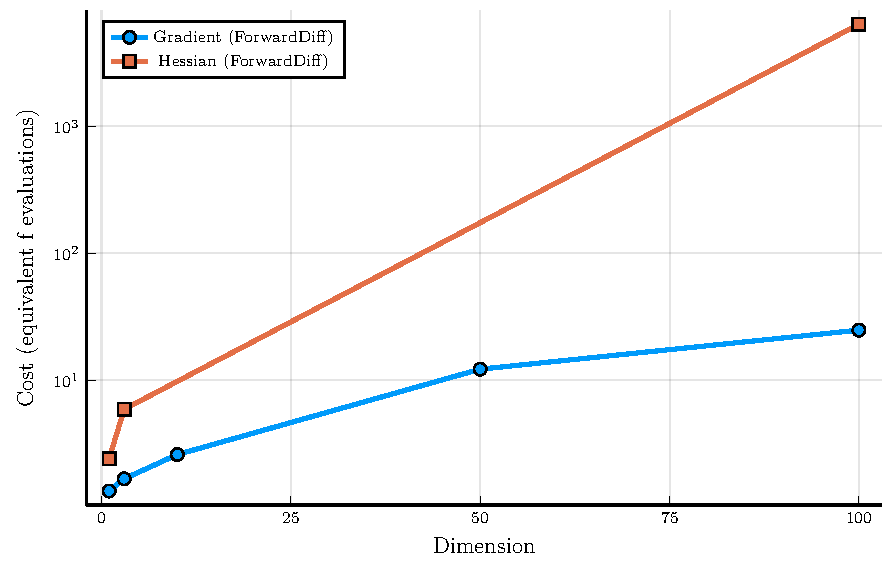
\includegraphics[width=0.8\linewidth]{ffjm2fig1.pdf}
	\caption{Cost, in equivalent evaluations of $f$, of computing the gradient and the Hessian of the PDE solver's objective by automatic differentiation, as a function of the problem dimension.}
	\label{fig:tempo_derivada}
\end{figure}
\FloatBarrier

At dimension 100, Figure~\ref{fig:tempo_derivada} shows that a single gradient evaluation already costs about as much as 25 evaluations of $f$, while a single Hessian evaluation costs more than 6400 evaluations of $f$.

For this reason, we need to make full use of the information already available to us, particularly the gradient, in order to solve this problem efficiently.







\section{Computational tests}
\label{sec:computational-tests}

\noindent
In this section we evaluate the performance of Algorithm~\ref{complexity}.1
and compare it against a classical
sum-of-squares approach. We run two types of tests. In the first, we
consider the MGH (Mor\'e, Garbow, and Hillstrom) sum-of-squares test
problems \cite{MoreGarbowHillstrom1981}, a benchmark of 34 classical
problems. This part is important to us because it helps us settle on a
good solver and Hessian approximation. In the second part, we solve a
hydraulic problem in which we need to estimate a coefficient of a PDE
called the Saint-Venant equation.


\subsection{Algorithm~\ref{complexity}.1 for MGH problems}
\label{sec:mgh-problems}

\noindent
Algorithm~\ref{complexity}.1 minimizes $f(x) = \frac{1}{2}\|F(x)\|_2^2$ by minimizing, at each iteration, a local quartic model of the
residuals in place of a line search. Following Algorithm~\ref{complexity}.1 (Eq.~(21)),
the step $s$ at iteration $k$ solves
\[
M_k(s) = \sigma\|s\|_2^2 + \frac{1}{2}\sum_{i=1}^m q_i(s)^2, \qquad
q_i(s) = f_i(x_k) + \nabla f_i(x_k)^\top s + \frac{1}{2} s^\top H_i s,
\]
where $f_i$ and $\nabla f_i$ are the $i$-th residual and its gradient at
$x_k$ (Section~3), $H_i$ is the current quasi-Newton approximation to its
Hessian. Four further variants are
compared in Table~\ref{tab:hessian-models}, and $\sigma\|s\|_2^2$
is the Levenberg-Marquardt-style regularization of Algorithm~\ref{complexity}.1 that
damps the step in place of a line search. The candidate $x_k + s$ is
checked for feasibility as in Step~3 (Eq.~\ref{feasi}). Acceptance then uses the
ratio $\rho_k$ between the actual and the model-predicted reduction in
$f$, a refinement of Algorithm~\ref{complexity}.1's simpler decrease test (Eq.~(25)),
accepting whenever $\rho_k \ge \eta_1$ for a fixed threshold $\eta_1$.

The implementation tested below uses the regularization update of
Eq.~(\ref{upsig}) with the following parameters. The first iteration starts at
$\sigma = 1$. Each accepted step divides $\sigma$ by a fixed factor
$\sigma_{grow} = 10$, and each rejected step, as in Eq.~(30), multiplies
$\sigma$ by the same factor $\sigma_{grow} = 10$ and re-solves the
subproblem at the same point, until a step is accepted. Between outer
iterations, $\sigma$ always carries over from the previous one rather
than being reset. The floor $\sigma_{\min} = 10^{-8}$ and the ceiling
$\sigma_{\max} = 10^{12}$ are used purely for numerical stability,
preventing $\sigma$ from underflowing or overflowing over the course of a
run.

Every run reported below stops under one of three point-wise criteria,
evaluated with the same default tolerances for Algorithm~\ref{complexity}.1 and for
Optim.jl's \texttt{BFGS} \cite{Mogensen2018} (kept equal so the comparison
is fair):
\begin{itemize}
	\item \textbf{Gradient}: the gradient norm reaches $\|\nabla f\| \le 10^{-8}$. This is a genuine first-order stationary point (reported as \texttt{grad\_conv} for both Algorithm~\ref{complexity}.1 and BFGS in the tables below).
	\item \textbf{Step}: the last step has (numerically) zero length. The solver stalls and stops making progress (reported as \texttt{step\_conv} for both Algorithm~\ref{complexity}.1 and BFGS).
	\item \textbf{Function}: the objective value does not change between two consecutive iterations. The iterate is stuck on a plateau (reported as \texttt{func\_conv} for both Algorithm~\ref{complexity}.1 and BFGS).
	\item \textbf{Stalled}: Algorithm~\ref{complexity}.1's regularization parameter exceeded its
	ceiling, that is, $\sigma > 10^{12}$ (reported as \texttt{reg\_stalled}. BFGS has no equivalent criterion).
\end{itemize}
Gradient, Step, and Function use the same name for both methods by
construction: BFGS's own status is classified by checking
\texttt{Optim.g\_converged}, then \texttt{Optim.x\_converged}, then
\texttt{Optim.f\_converged} on its result, in that order, so the two
methods can be compared under one shared vocabulary instead of each
reporting its own native termination code.
%A run that exhausts the iteration budget without meeting any of the first
%three would be reported separately as \emph{not converged}. This case
%does not appear in Tables~\ref{tab:hessian-models} and
%\ref{tab:psb-vs-sr1} below, but it does in
%Table~\ref{tab:psb-vs-bfgs}. Algorithm~\ref{complexity}.1 (PSB) now stops under the
%\textbf{Stalled} criterion on MGH10, MGH16, and MGH31 (the same three
%problems that previously stopped under Step/Function; see the
%discussion after that table).

Table~\ref{tab:hessian-models} compares the six Algorithm~\ref{complexity}.1 Hessian-update
models, each run independently on the 34 MGH least-squares problems
\cite{MoreGarbowHillstrom1981}. Its ``Converged (gradient)'' column counts
how many of the 34 problems stopped under the gradient criterion. The
remaining columns are mean~$\pm$~standard deviation over the 34 problems.
Each model keeps its own set of matrices $H_i \approx \nabla^2 f_i(x_k)$,
$i=1,\ldots,m$, updated at every accepted step from $s = x_{k+1}-x_k$ and
$y_i = \nabla f_i(x_{k+1}) - \nabla f_i(x_k)$:
\begin{itemize}
	\item \textbf{BFGS}: the classical rank-two secant update
	\cite{Broyden1970,Fletcher1970,Goldfarb1970,Shanno1970,NocedalWright2006} (Eq.~(19)),
	\[
	H_i \leftarrow H_i - \frac{H_i s\,s^T H_i}{s^T H_i s} + \frac{y_i y_i^T}{s^T y_i}.
	\]
	\item \textbf{SR1}: the symmetric rank-one update \cite{NocedalWright2006} (Eq.~(20)),
	\[
	H_i \leftarrow H_i + \frac{(y_i - H_i s)(y_i - H_i s)^T}{(y_i - H_i s)^T s}.
	\]
	\item \textbf{DW} (Dennis-Wolkowicz \cite{DennisWolkowicz1993}, Theorem
	4.5(iii)): a Broyden-class update that adds a third, symmetrizing
	rank-one term to the BFGS pair,
	\[
	H_i \leftarrow H_i - \frac{H_i s\,s^T H_i}{s^T H_i s} + \frac{y_i y_i^T}{s^T y_i}
	+ (s^T y_i)\, w_i w_i^T, \qquad
	w_i = \frac{y_i}{s^T y_i} - \frac{H_i s}{s^T H_i s}.
	\]
	\item \textbf{PSB} (Powell-Symmetric-Broyden \cite{Powell1970}): a
	rank-two update that does not preserve positive definiteness (like
	SR1),
	\[
	H_i \leftarrow H_i + \frac{(y_i - H_i s)s^T + s(y_i - H_i s)^T}{s^T s}
	- \frac{s^T(y_i - H_i s)}{(s^T s)^2}\, s s^T.
	\]
\end{itemize}

\begin{table}[htbp]
	\centering
	\caption{Comparison of the Algorithm~\ref{complexity}.1 Hessian-update models on the 34 MGH problems.}
	\label{tab:hessian-models}
	\begin{tabular}{l r r r r r}
		\toprule
		Model & Converged (gradient) & Iterations & Func.\ evals & Grad.\ evals & Time (s) \\
		\midrule
		BFGS & 29/34 & $56.88 \pm 188.25$ & $99.97 \pm 351.85$ & $57.88 \pm 188.25$ & $2.071 \pm 6.121$ \\
		SR1 & 32/34 & $23.12 \pm 54.84$ & $44.32 \pm 112.92$ & $24.12 \pm 54.84$ & $0.934 \pm 2.992$ \\
		DW & 29/34 & $56.12 \pm 181.91$ & $103.24 \pm 351.45$ & $57.12 \pm 181.91$ & $1.865 \pm 5.942$ \\
		PSB & 31/34 & $15.68 \pm 22.53$ & $31.38 \pm 53.44$ & $16.68 \pm 22.53$ & $0.424 \pm 0.919$ \\
		\bottomrule
	\end{tabular}
\end{table}

\FloatBarrier

\noindent
PSB and SR1 are the two best models. Together they solve the most problems
under the gradient criterion, and PSB in particular does so with by far the
fewest iterations, evaluations, and execution time on average
(Table~\ref{tab:hessian-models}). SR1 nonetheless certifies gradient
convergence on one more problem than PSB (32/34 against 31/34). To see
exactly where they disagree, Table~\ref{tab:psb-vs-sr1} isolates the three
problems on which at least one of the two methods does not stop under the
gradient criterion.

{\footnotesize
	\begin{longtable}{l l S[table-format=1.3e2] S[table-format=1.3e2] r r >{\raggedright\arraybackslash}p{2.2cm}}
		\caption{Algorithm~\ref{complexity}.1 (PSB) vs.\ Algorithm~\ref{complexity}.1 (SR1): per-problem comparison on the MGH problems.}
		\label{tab:psb-vs-sr1} \\
		\toprule
		Problem & Method & {$f$} & {$\|\nabla f\|$} & {Func.\ evals} & {Grad.\ evals} & Criterion \\
		\midrule
		\endfirsthead
		\caption[]{(continued)} \\
		\toprule
		Problem & Method & {$f$} & {$\|\nabla f\|$} & {Func.\ evals} & {Grad.\ evals} & Criterion \\
		\midrule
		\endhead
		\midrule
		\multicolumn{7}{r}{\textit{continued on next page}} \\
		\endfoot
		\bottomrule
		\endlastfoot
		MGH10 & Algorithm~\ref{complexity}.1 (PSB) & 4.397293e+01 & 5.754922e-05 & 299 & 127 & \texttt{step\_conv} \\
		MGH10 & Algorithm~\ref{complexity}.1 (SR1) & 4.397293e+01 & 5.500886e-02 & 297 & 125 & \texttt{step\_conv} \\
		\midrule
		MGH16 & Algorithm~\ref{complexity}.1 (PSB) & 4.291110e+04 & 9.258506e-05 & 98 & 36 & \texttt{func\_conv} \\
		MGH16 & Algorithm~\ref{complexity}.1 (SR1) & 4.291110e+04 & 6.255963e-05 & 44 & 9 & \texttt{func\_conv} \\
		\midrule
		MGH31 & Algorithm~\ref{complexity}.1 (PSB) & 1.528639e+00 & 2.527165e-08 & 62 & 21 & \texttt{func\_conv} \\
		MGH31 & Algorithm~\ref{complexity}.1 (SR1) & 1.528639e+00 & 4.387102e-09 & 44 & 29 & \texttt{grad\_conv} \\
\end{longtable}}
\FloatBarrier

\noindent
On MGH10 and MGH16, neither model reaches the gradient criterion, both
stall under the step and function criteria, respectively, at essentially
the same objective value, although Algorithm~\ref{complexity}.1 with PSB reaches a smaller
gradient norm on MGH10. For this reason, PSB is the best
choice between the two approaches when weighing cost against benefit.




Table~\ref{tab:ffjm2-subproblem-solvers} repeats the comparison, but now
running Algorithm~\ref{complexity}.1 in full with PSB model on the same 34
problems. Newton/BFGS/BOBYQA solve
only the small quartic model at each outer iteration, exactly as Algorithm~\ref{complexity}.1
uses them, instead of standing in as the whole optimizer. ``Newton''
here is the exact Newton step on the
quartic subproblem, computed via the Ipopt interior-point solver.



Function and gradient evaluations here count only the calls to the real
residual and Jacobian made by Algorithm~\ref{complexity}.1's outer loop. The
internal solver's own work on the quartic surrogate is tracked
separately, since evaluating the true function and its derivative is
considerably more expensive than evaluating the model. Because we are
solving a quartic (rather than a quadratic) problem, we use a multistart
method to search for a global optimum. At each outer iteration $k$, $100$
random points are drawn from a ball $B(0, \max\{1, d_{k-1}\})$. Using the
default multistart setting for every method would be impractical across
all 34 problems in this table.

\begin{table}[htbp]
	\centering
	\caption{Algorithm~\ref{complexity}.1 (PSB), varying only \texttt{model\_solver}, on the 34 MGH problems.}
	\label{tab:ffjm2-subproblem-solvers}
	\resizebox{\textwidth}{!}{%
		\begin{tabular}{l r r r r r}
			\toprule
			Method & $f$ & Converged (gradient) & Iterations & Func.\ evals & Grad.\ evals \\
			\midrule
			Algorithm~\ref{complexity}.1 (PSB, Newton) & $1.29\times10^{3} \pm 7.36\times10^{3}$ & 31/34 & $15.12 \pm 21.90$ & $30.21 \pm 49.59$ & $16.12 \pm 21.90$ \\
			Algorithm~\ref{complexity}.1 (PSB, BFGS) & $1.29\times10^{3} \pm 7.36\times10^{3}$ & 31/34 & $15.26 \pm 21.99$ & $30.26 \pm 48.63$ & $16.26 \pm 21.99$ \\
			Algorithm~\ref{complexity}.1 (PSB, BOBYQA) & $1.29\times10^{3} \pm 7.36\times10^{3}$ & 30/34 & $39.74 \pm 108.86$ & $57.68 \pm 127.48$ & $40.74 \pm 108.86$ \\
			\bottomrule
		\end{tabular}%
	}
\end{table}
\FloatBarrier

\noindent
Newton and BFGS are essentially indistinguishable
(31/34, within $1\%$ of each other on every column), and even BOBYQA, which needed an order of magnitude more evaluations and converged on only
10/34 when applied directly to the raw residual, falls behind by only
one problem (30/34) and roughly $2.6\times$ more outer iterations on
average. This distinction matters because evaluating the derivative can
sometimes cost more than $2.6\times$ what evaluating the objective
function costs. Since Newton achieves the best
performance among the three, we adopt it as the model solver
used throughout the rest of this work.




\needspace{10\baselineskip}
\subsection{Sum of square problem BFGS configuration}

We now consider a different configuration than the average BFGS method. We do this because the default line search, generally the Hager-Zhang line search, evaluates the derivative of the function many times. For this reason, we now test different classical line searches for the BFGS method. Table~\ref{tab:bfgs-linesearches} checks some line searches for
\texttt{Optim.BFGS} on the same 34 MGH problems with four line searches. Hager and Zhang (\texttt{Optim.jl}'s default), a
minimalist backtracking with Armijo condition, and Backtracking
with quadratic (order 2) and cubic (order 3) interpolation. ``Converged
(gradient)'' counts how many of the 34 problems stopped under the gradient
criterion. The remaining columns are mean~$\pm$~standard deviation over
all 34 problems (including the ones that stopped under a different
criterion).

\begin{table}[htbp]
	\centering
	\caption{Comparison of line searches for Optim.jl's BFGS on the 34 MGH problems.}
	\label{tab:bfgs-linesearches}
	\resizebox{\textwidth}{!}{%
		\begin{tabular}{l r r r r r}
			\toprule
			Method & $f$ & Converged (gradient) & Iterations & Func.\ evals & Grad.\ evals \\
			\midrule
			Hager-Zhang & $1.29\times10^{3} \pm 7.36\times10^{3}$ & 33/34 & $66.91 \pm 120.92$ & $107.82 \pm 206.62$ & $107.82 \pm 206.62$ \\
			Backtracking & $2.49\times10^{7} \pm 1.45\times10^{8}$ & 30/34 & $51.56 \pm 93.74$ & $89.62 \pm 131.90$ & $52.47 \pm 93.75$ \\
			Backtracking (order 2) & $1.29\times10^{3} \pm 7.36\times10^{3}$ & 32/34 & $61.59 \pm 99.26$ & $86.74 \pm 134.56$ & $62.56 \pm 99.17$ \\
			Backtracking (order 3) & $1.29\times10^{3} \pm 7.36\times10^{3}$ & 31/34 & $56.91 \pm 89.47$ & $84.91 \pm 132.01$ & $57.85 \pm 89.33$ \\
			\bottomrule
		\end{tabular}%
	}
\end{table}
\FloatBarrier

\noindent
Hager-Zhang converges by gradient on the most problems (33/34) but at the
highest average cost. Backtracking is a cheap line search, but its value of $f$ and its convergence rate per
problem are not as good on average (30/34). Backtracking order 2 and order 3 have similar results. Although Backtracking order 3 has slightly fewer evaluations, Backtracking order 2 found gradient convergence on 32/34 problems. For this reason, we choose Backtracking order 2 to compare with our approach.


%
%
%\newpage
%A second aside: FFJM2's quartic subproblem (Section~2, Eq.~(18)/(21)) is
%solved internally by Ipopt, but the paper's Algorithm 4.1 does not require
%that particular choice. Table~\ref{tab:subproblem-solvers} checks how the
%four solvers already available as \texttt{model\_solver} in \texttt{ffjm2}
%--- Ipopt, BFGS (backtracking, same as above), BOBYQA, and MADS --- fare
%when applied \emph{directly} to $0.5\|F(x)\|^2$ on the 34 MGH problems
%(i.e., as if each one were, on its own, the whole optimizer, not just the
%subproblem solver inside FFJM2's outer loop). Same columns as
%Table~\ref{tab:bfgs-linesearches}; BOBYQA and MADS are derivative-free, so
%their gradient-evaluation count is always $0$ and ``Converged (gradient)''
%for them instead counts $\|\nabla f\|\le10^{-8}$ checked \emph{after} the
%solver stops (Ipopt and BFGS report their own gradient-based termination
%directly).
%
%\begin{table}[htbp]
%	\centering
%	\caption{Comparison of the solvers available for FFJM2's internal
	%		subproblem, applied directly to $0.5\|F(x)\|^2$ on the 34 MGH problems.}
%	\label{tab:subproblem-solvers}
%	\resizebox{\textwidth}{!}{%
	%		\begin{tabular}{l r r r r r}
		%			\toprule
		%			Method & $f$ & Converged (gradient) & Iterations & Func.\ evals & Grad.\ evals \\
		%			\midrule
		%			Ipopt & $1.88\times10^{5} \pm 1.09\times10^{6}$ & 32/34 & $69.53 \pm 103.06$ & $424.62 \pm 803.24$ & $71.53 \pm 103.06$ \\
		%			BFGS (backtracking) & $1.29\times10^{3} \pm 7.36\times10^{3}$ & 32/34 & $61.59 \pm 99.26$ & $86.74 \pm 134.56$ & $62.56 \pm 99.17$ \\
		%			BOBYQA & $1.47\times10^{10} \pm 8.56\times10^{10}$ & 10/34 & $572.71 \pm 699.05$ & $572.71 \pm 699.05$ & $0.00 \pm 0.00$ \\
		%			MADS & $1.47\times10^{10} \pm 8.56\times10^{10}$ & 0/34 & $986.82 \pm 594.53$ & $986.82 \pm 594.53$ & $0.00 \pm 0.00$ \\
		%			\bottomrule
		%		\end{tabular}%
	%	}
%\end{table}
%
%\noindent
%Ipopt and BFGS are essentially tied on reliability (32/34) and land within
%a factor of $2$ of each other on iterations and gradient evaluations, but
%Ipopt needs about $5\times$ more function evaluations on average (it
%solves a full barrier subproblem at each outer iteration). BOBYQA and MADS
%are far behind on both counts: with no gradient to exploit, they need an
%order of magnitude more evaluations and still only certify gradient
%convergence on 10/34 (BOBYQA) or none at all (MADS) within the $2000$
%function-evaluation budget. As Table~\ref{tab:ffjm2-subproblem-solvers}
%below shows, this gap does \emph{not} carry over once these solvers are
%used the way FFJM2 actually uses them --- as the resolver of the small,
%cheap quartic model, rather than as the whole optimizer applied to the raw
%residual. As in Table~\ref{tab:bfgs-linesearches}, the mean/std of $f$
%is dominated by outliers rather than typical behavior, and here they point
%to a genuine methodological limitation of the box these two derivative-free
%solvers need (BOBYQA and MADS require finite bounds; both are given
%$x^0\pm\mathrm{bound\_radius}$, $\mathrm{bound\_radius}=\max(10^3,
%100\max(1,\|x^0\|))$): on MGH04, whose true minimizer is
%$x^*\approx(10^6,\,2\times10^{-6})$, this box does not even contain
%$x^*$ when $x^0=(1,1)$ gives $\mathrm{bound\_radius}=10^3$, so both solvers
%stall at the box boundary ($f\approx5.0\times10^{11}$, versus
%$\approx8\times10^{-28}$ for Ipopt/BFGS on the same problem) --- a box
%sized from $\|x^0\|$ alone cannot help when $x^*$ is orders of magnitude
%farther from $x^0$ than $x^0$ is from the origin. Ipopt's own outlier is
%different in kind: on MGH10 it converges (\texttt{LOCALLY\_SOLVED}) to a
%KKT point with $f\approx6.3\times10^6$, well above BFGS's
%$f\approx44$ on the same problem, i.e.\ a genuine bad local
%solution rather than a boundary artifact.

\subsection{Algorithm~\ref{complexity}.1 against BFGS with backtracking}

Algorithm~\ref{complexity}.1 (PSB) uses persistent decaying $\sigma$, a full Hessian reset on a bad
ratio, and $-\nabla f$+Armijo at $k=0$ and as a safeguard. The following
table compares it against BFGS with backtracking line search on the 34
MGH least-squares problems.

{\footnotesize
	\begin{longtable}{l l S[table-format=1.3e2] S[table-format=1.3e2] r r >{\raggedright\arraybackslash}p{2.2cm}}
		\caption{Algorithm~\ref{complexity}.1 (PSB) vs.\ BFGS (backtracking): per-problem comparison on the MGH problems.}
		\label{tab:psb-vs-bfgs} \\
		\toprule
		Problem & Method & {$f$} & {$\|\nabla f\|$} & {Func.\ evals} & {Grad.\ evals} & Criterion \\
		\midrule
		\endfirsthead
		\caption[]{(continued)} \\
		\toprule
		Problem & Method & {$f$} & {$\|\nabla f\|$} & {Func.\ evals} & {Grad.\ evals} & Criterion \\
		\midrule
		\endhead
		\midrule
		\multicolumn{7}{r}{\textit{continued on next page}} \\
		\endfoot
		\bottomrule
		\endlastfoot
		MGH01 & Algorithm~\ref{complexity}.1 (PSB) & 2.415715e-22 & 9.822188e-12 & 12 & 8 & \texttt{grad\_conv} \\
		MGH01 & BFGS (backtracking) & 1.981121e-22 & 3.687403e-10 & 53 & 40 & \texttt{grad\_conv} \\
		\midrule
		MGH02 & Algorithm~\ref{complexity}.1 (PSB) & 5.096567e-18 & 3.844849e-09 & 10 & 7 & \texttt{grad\_conv} \\
		MGH02 & BFGS (backtracking) & 1.106930e-26 & 2.198151e-12 & 15 & 11 & \texttt{grad\_conv} \\
		\midrule
		MGH03 & Algorithm~\ref{complexity}.1 (PSB) & 1.576836e-11 & 2.568219e-09 & 31 & 20 & \texttt{grad\_conv} \\
		MGH03 & BFGS (backtracking) & 5.053640e-30 & 2.830752e-10 & 233 & 174 & \texttt{grad\_conv} \\
		\midrule
		MGH04 & Algorithm~\ref{complexity}.1 (PSB) & 3.811648e-17 & 8.733972e-09 & 10 & 8 & \texttt{grad\_conv} \\
		MGH04 & BFGS (backtracking) & 9.860761e-32 & 4.440892e-10 & 40 & 14 & \texttt{grad\_conv} \\
		\midrule
		MGH05 & Algorithm~\ref{complexity}.1 (PSB) & 1.307511e-16 & 6.948485e-09 & 10 & 8 & \texttt{grad\_conv} \\
		MGH05 & BFGS (backtracking) & 2.500895e-22 & 1.079551e-10 & 22 & 19 & \texttt{grad\_conv} \\
		\midrule
		MGH06 & Algorithm~\ref{complexity}.1 (PSB) & 1.010000e+03 & 1.161571e-28 & 11 & 2 & \texttt{grad\_conv} \\
		MGH06 & BFGS (backtracking) & 1.010000e+03 & 1.161571e-28 & 10 & 2 & \texttt{grad\_conv} \\
		\midrule
		MGH07 & Algorithm~\ref{complexity}.1 (PSB) & 1.492293e-17 & 6.034835e-09 & 17 & 10 & \texttt{grad\_conv} \\
		MGH07 & BFGS (backtracking) & 5.236320e-19 & 5.028697e-09 & 41 & 30 & \texttt{grad\_conv} \\
		\midrule
		MGH08 & Algorithm~\ref{complexity}.1 (PSB) & 4.107439e-03 & 4.903415e-10 & 12 & 9 & \texttt{grad\_conv} \\
		MGH08 & BFGS (backtracking) & 4.107439e-03 & 7.394161e-10 & 34 & 28 & \texttt{grad\_conv} \\
		\midrule
		MGH09 & Algorithm~\ref{complexity}.1 (PSB) & 5.639664e-09 & 7.549518e-11 & 9 & 7 & \texttt{grad\_conv} \\
		MGH09 & BFGS (backtracking) & 5.639664e-09 & 1.552131e-09 & 6 & 5 & \texttt{grad\_conv} \\
		\midrule
		MGH10 & Algorithm~\ref{complexity}.1 (PSB) & 4.397293e+01 & 1.204293e-05 & 276 & 122 & \texttt{reg\_stalled} \\
		MGH10 & BFGS (backtracking) & 4.397293e+01 & 2.281500e+00 & 552 & 386 & \texttt{step\_conv} \\
		\midrule
		MGH11 & Algorithm~\ref{complexity}.1 (PSB) & 5.960004e-21 & 3.251504e-13 & 26 & 17 & \texttt{grad\_conv} \\
		MGH11 & BFGS (backtracking) & 2.268388e-20 & 7.169397e-10 & 50 & 42 & \texttt{grad\_conv} \\
		\midrule
		MGH12 & Algorithm~\ref{complexity}.1 (PSB) & 3.799377e-18 & 3.814938e-10 & 14 & 11 & \texttt{grad\_conv} \\
		MGH12 & BFGS (backtracking) & 1.579764e-21 & 3.202002e-11 & 53 & 41 & \texttt{grad\_conv} \\
		\midrule
		MGH13 & Algorithm~\ref{complexity}.1 (PSB) & 5.156722e-12 & 9.613609e-09 & 12 & 9 & \texttt{grad\_conv} \\
		MGH13 & BFGS (backtracking) & 1.566490e-14 & 3.607786e-09 & 55 & 45 & \texttt{grad\_conv} \\
		\midrule
		MGH14 & Algorithm~\ref{complexity}.1 (PSB) & 9.424359e-19 & 8.234967e-10 & 11 & 7 & \texttt{grad\_conv} \\
		MGH14 & BFGS (backtracking) & 3.521535e-22 & 5.460933e-10 & 44 & 31 & \texttt{grad\_conv} \\
		\midrule
		MGH15 & Algorithm~\ref{complexity}.1 (PSB) & 1.537528e-04 & 9.059854e-09 & 38 & 22 & \texttt{grad\_conv} \\
		MGH15 & BFGS (backtracking) & 1.537528e-04 & 4.132861e-10 & 39 & 33 & \texttt{grad\_conv} \\
		\midrule
		MGH16 & Algorithm~\ref{complexity}.1 (PSB) & 4.291110e+04 & 6.530587e-05 & 91 & 37 & \texttt{reg\_stalled} \\
		MGH16 & BFGS (backtracking) & 4.291110e+04 & 2.831466e-05 & 72 & 26 & \texttt{func\_conv} \\
		\midrule
		MGH17 & Algorithm~\ref{complexity}.1 (PSB) & 2.732447e-05 & 8.377671e-09 & 24 & 12 & \texttt{grad\_conv} \\
		MGH17 & BFGS (backtracking) & 2.732447e-05 & 8.227669e-09 & 90 & 59 & \texttt{grad\_conv} \\
		\midrule
		MGH18 & Algorithm~\ref{complexity}.1 (PSB) & 1.002042e-18 & 1.650363e-11 & 58 & 34 & \texttt{grad\_conv} \\
		MGH18 & BFGS (backtracking) & 2.827825e-03 & 1.276728e-08 & 44 & 41 & \texttt{grad\_conv} \\
		\midrule
		MGH19 & Algorithm~\ref{complexity}.1 (PSB) & 4.383556e-02 & 9.198492e-09 & 115 & 59 & \texttt{grad\_conv} \\
		MGH19 & BFGS (backtracking) & 1.373773e-01 & 8.291793e-10 & 147 & 113 & \texttt{grad\_conv} \\
		\midrule
		MGH20 & Algorithm~\ref{complexity}.1 (PSB) & 1.143835e-03 & 1.841972e-09 & 13 & 10 & \texttt{grad\_conv} \\
		MGH20 & BFGS (backtracking) & 1.143835e-03 & 7.070265e-09 & 49 & 39 & \texttt{grad\_conv} \\
		\midrule
		MGH21 & Algorithm~\ref{complexity}.1 (PSB) & 2.415715e-21 & 3.106049e-11 & 12 & 8 & \texttt{grad\_conv} \\
		MGH21 & BFGS (backtracking) & 4.792661e-18 & 1.495834e-09 & 228 & 150 & \texttt{grad\_conv} \\
		\midrule
		MGH22 & Algorithm~\ref{complexity}.1 (PSB) & 4.516652e-14 & 2.795657e-10 & 13 & 10 & \texttt{grad\_conv} \\
		MGH22 & BFGS (backtracking) & 1.653367e-13 & 1.561713e-08 & 136 & 112 & \texttt{grad\_conv} \\
		\midrule
		MGH23 & Algorithm~\ref{complexity}.1 (PSB) & 1.124989e-05 & 2.279978e-09 & 13 & 10 & \texttt{grad\_conv} \\
		MGH23 & BFGS (backtracking) & 1.124989e-05 & 1.205331e-08 & 87 & 68 & \texttt{grad\_conv} \\
		\midrule
		MGH24 & Algorithm~\ref{complexity}.1 (PSB) & 1.728411e-06 & 1.740229e-09 & 37 & 22 & \texttt{grad\_conv} \\
		MGH24 & BFGS (backtracking) & 1.728411e-06 & 6.288297e-09 & 588 & 450 & \texttt{grad\_conv} \\
		\midrule
		MGH25 & Algorithm~\ref{complexity}.1 (PSB) & 7.395571e-32 & 3.845925e-16 & 13 & 6 & \texttt{grad\_conv} \\
		MGH25 & BFGS (backtracking) & 6.843630e-26 & 7.268618e-12 & 23 & 16 & \texttt{grad\_conv} \\
		\midrule
		MGH26 & Algorithm~\ref{complexity}.1 (PSB) & 1.397528e-05 & 2.997834e-09 & 27 & 16 & \texttt{grad\_conv} \\
		MGH26 & BFGS (backtracking) & 1.397528e-05 & 1.106362e-08 & 36 & 34 & \texttt{grad\_conv} \\
		\midrule
		MGH27 & Algorithm~\ref{complexity}.1 (PSB) & 2.240730e-16 & 1.941231e-09 & 11 & 8 & \texttt{grad\_conv} \\
		MGH27 & BFGS (backtracking) & 5.734697e-20 & 3.689878e-09 & 20 & 17 & \texttt{grad\_conv} \\
		\midrule
		MGH28 & Algorithm~\ref{complexity}.1 (PSB) & 2.223149e-15 & 6.931523e-09 & 10 & 8 & \texttt{grad\_conv} \\
		MGH28 & BFGS (backtracking) & 2.533828e-16 & 1.086349e-08 & 26 & 18 & \texttt{grad\_conv} \\
		\midrule
		MGH29 & Algorithm~\ref{complexity}.1 (PSB) & 1.130540e-22 & 1.906829e-11 & 8 & 7 & \texttt{grad\_conv} \\
		MGH29 & BFGS (backtracking) & 9.104593e-19 & 1.563296e-09 & 8 & 8 & \texttt{grad\_conv} \\
		\midrule
		MGH30 & Algorithm~\ref{complexity}.1 (PSB) & 7.642460e-27 & 3.456063e-13 & 10 & 7 & \texttt{grad\_conv} \\
		MGH30 & BFGS (backtracking) & 1.965544e-19 & 4.026641e-09 & 46 & 23 & \texttt{grad\_conv} \\
		\midrule
		MGH31 & Algorithm~\ref{complexity}.1 (PSB) & 1.528639e+00 & 4.173205e-08 & 49 & 18 & \texttt{reg\_stalled} \\
		MGH31 & BFGS (backtracking) & 1.340110e+00 & 4.482312e-09 & 78 & 43 & \texttt{grad\_conv} \\
		\midrule
		MGH32 & Algorithm~\ref{complexity}.1 (PSB) & 5.000000e+00 & 3.845925e-16 & 3 & 2 & \texttt{grad\_conv} \\
		MGH32 & BFGS (backtracking) & 5.000000e+00 & 5.578802e-16 & 2 & 2 & \texttt{grad\_conv} \\
		\midrule
		MGH33 & Algorithm~\ref{complexity}.1 (PSB) & 2.317073e+00 & 6.326298e-11 & 12 & 5 & \texttt{grad\_conv} \\
		MGH33 & BFGS (backtracking) & 2.317073e+00 & 1.423632e-10 & 13 & 5 & \texttt{grad\_conv} \\
		\midrule
		MGH34 & Algorithm~\ref{complexity}.1 (PSB) & 3.067568e+00 & 1.552202e-10 & 9 & 2 & \texttt{grad\_conv} \\
		MGH34 & BFGS (backtracking) & 3.067568e+00 & 2.134352e-10 & 9 & 2 & \texttt{grad\_conv} \\
\end{longtable}}
\FloatBarrier

\noindent
Across the 34 problems, the two methods usually agree closely on the final
objective value, but differ sharply in cost. Algorithm~\ref{complexity}.1 (PSB) needs far fewer
function and gradient evaluations than BFGS on most problems (see
Table~\ref{tab:psb-vs-bfgs}). MGH10 shows how hard some of these problems
are. Neither method certifies gradient convergence there, and both land on
essentially the same objective value ($f\approx43.97$), yet Algorithm~\ref{complexity}.1 still
reaches a far smaller gradient norm than BFGS ($\|\nabla f\|\approx
1.2\times10^{-5}$ against $\approx2.28$), using half the function
evaluations and under a third of the gradient evaluations. MGH18 shows the
opposite kind of gap. Although both methods stop under the gradient
criterion, Algorithm~\ref{complexity}.1 reaches essentially zero ($f\approx1.0\times10^{-18}$)
while BFGS settles for a distinctly larger value ($f\approx2.8\times
10^{-3}$). A small gradient norm does not always mean the same
stationary point.

The boxplot below compares the two approaches directly and uses the
Mann-Whitney U test \cite{MannWhitney1947} to check whether the difference between them is
statistically significant.

\begin{figure}[htbp]
	\centering
	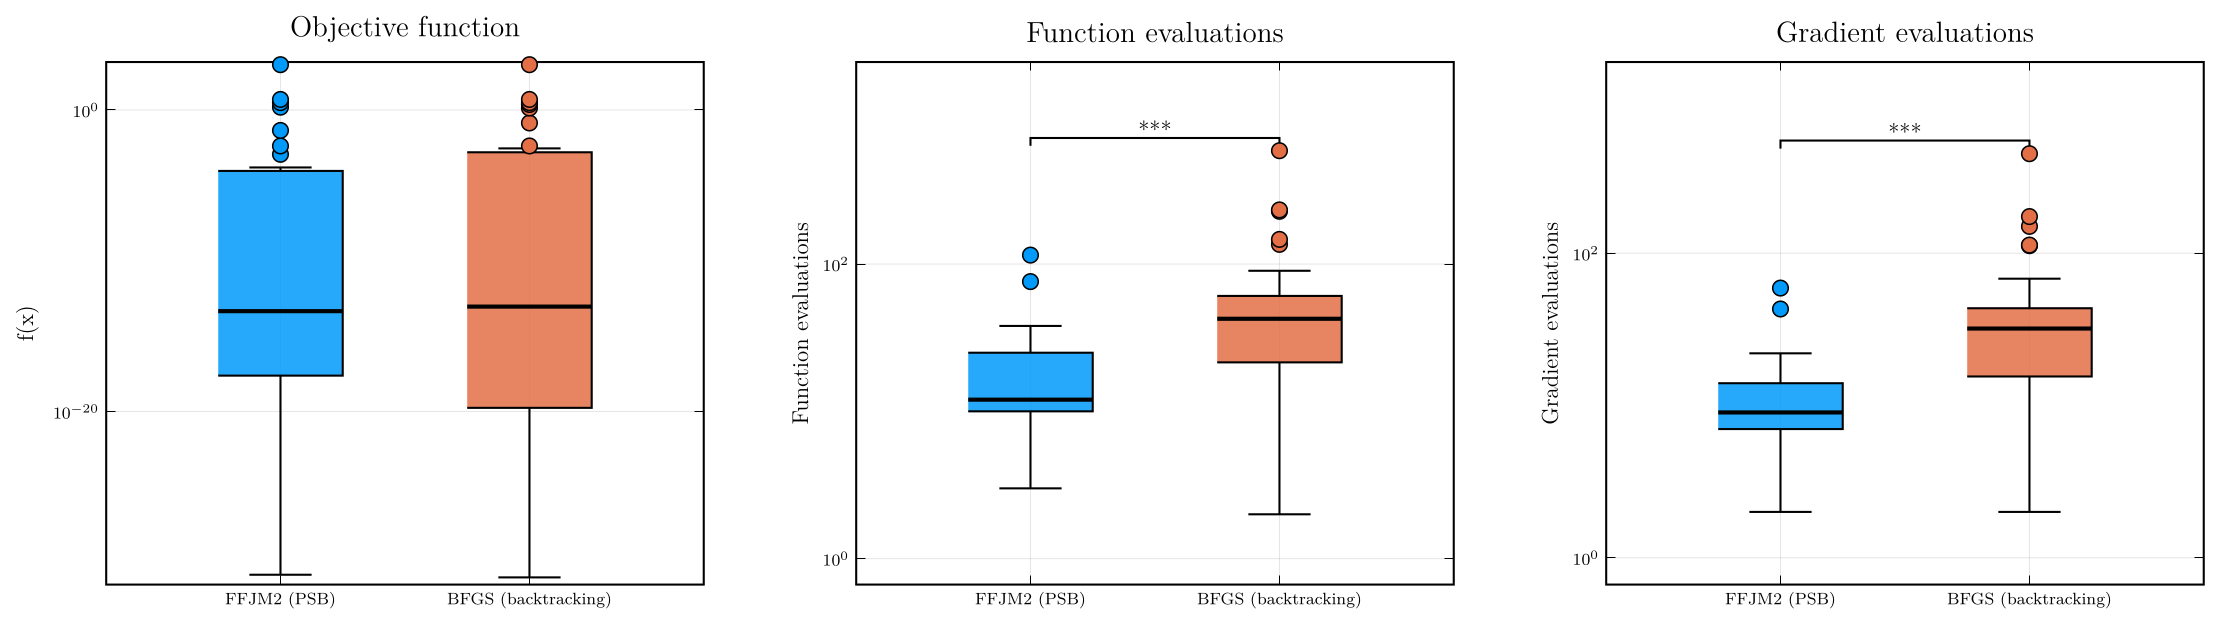
\includegraphics[width=\textwidth]{ffjm2fig2.png}
	\caption{Comparison of Algorithm~\ref{complexity}.1 (PSB), called \texttt{ffjm2}, vs.\ BFGS (backtracking) on the MGH
		problems, restricted to runs where both methods converged by
		gradient norm. Final
		$f$ value, function evaluations, and gradient evaluations. Stars
		indicate significance under the Mann-Whitney U test ($p < 0.05$:
		{*}; $p < 0.01$: {**}; $p < 0.001$: {***}).}
	\label{fig:boxplot-ffjm2-bfgs}
\end{figure}

\FloatBarrier

As Figure~\ref{fig:boxplot-ffjm2-bfgs} shows, the objective function values
are not very different between the two methods. The p-value confirms
neither achieves a significantly better result. Function evaluations and
gradient evaluations, however, are different, and the p-value confirms
this difference is significant. Algorithm~\ref{complexity}.1 therefore performs better than
BFGS in this respect, reaching a comparable solution at a much lower cost.

The boxplot above is restricted to the subset of problems where both
methods converge by gradient norm. To compare the two methods over all 34
problems, Figure~\ref{fig:performance-profiles} shows the performance
profile of Dolan and Mor\'e \cite{DolanMore2002} for the final objective
value, function evaluations, and gradient evaluations. For each problem, a method's ratio $r$ is its evaluation
count divided by the smaller of the two methods' counts on that same
problem, so the faster method has $r=1$. A run that does not converge by
gradient norm counts as a failure, with $r=\infty$ (a problem on which
neither method converges by gradient norm counts as a mutual failure,
$r=\infty$ for both, still included in the 34). The curve $\rho_s(\tau)$ is the
fraction of the 34 problems on which method $s$'s ratio is at most $\tau$,
plotted against $\log_2\tau$: $\rho_s(1)$ is therefore the fraction of
problems on which $s$ is the faster (or tied) method, and $\rho_s(\tau)$
as $\tau\to\infty$ approaches $s$'s overall convergence rate, independent
of cost. 


\begin{figure}[htbp]
	\centering
	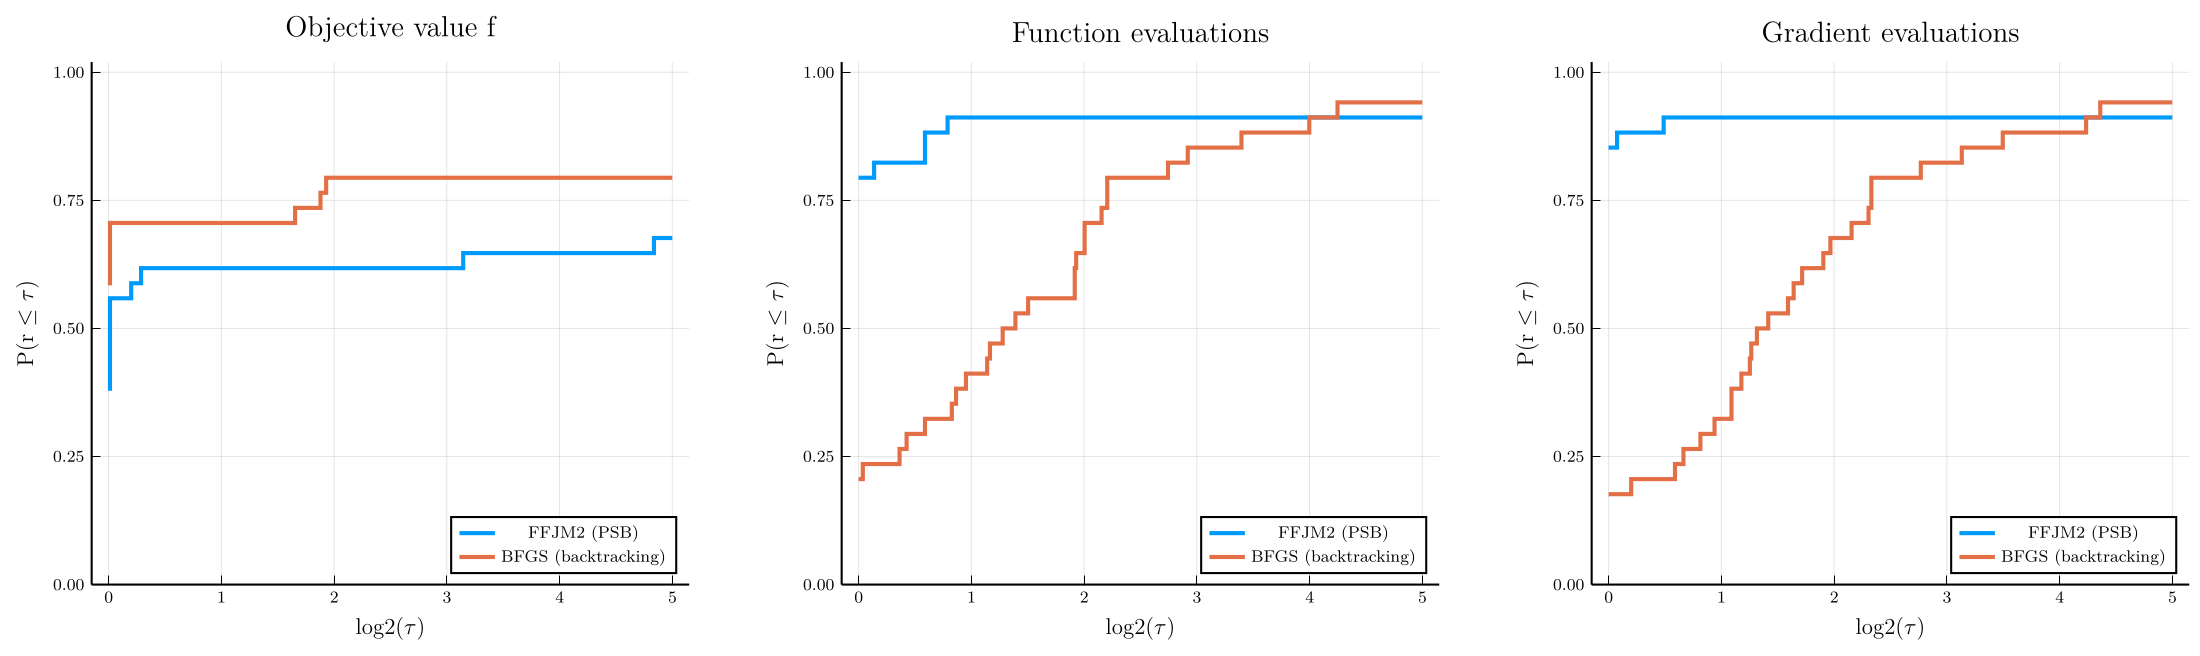
\includegraphics[width=\textwidth]{ffjm2fig3.png}
	\caption{Performance profile \cite{DolanMore2002} of Algorithm~\ref{complexity}.1 (PSB), called \texttt{ffjm2},
		vs.\ BFGS (backtracking) on all 34 MGH problems, for the final
		objective value (left), function evaluations (middle), and gradient
		evaluations (right). $\rho_s(\tau)$ is the fraction of problems on
		which method $s$'s cost (final $f$ value, function evaluations, or
		gradient evaluations, matching the panel) is at most $\tau$ times
		the smaller of the two methods' costs on that problem, plotted
		against $\log_2\tau$. A run that does not converge by gradient norm
		counts as a failure.}
	\label{fig:performance-profiles}
\end{figure}

\FloatBarrier

Looking only at the objective value in Figure~\ref{fig:performance-profiles},
BFGS comes out ahead, the better (or tied) method on close to 59\% of the
34 problems against 38\% for Algorithm~\ref{complexity}.1. Table~\ref{tab:psb-vs-bfgs}
and Figure~\ref{fig:boxplot-ffjm2-bfgs}, however, already showed that this
difference in objective value is not statistically significant. The
Mann-Whitney test does not treat it as a real gap in solution quality
between the two methods. For function and gradient evaluations, by
contrast, Algorithm~\ref{complexity}.1 is the better (or tied) method on
about 80\% of the 34 problems, and that difference \emph{is} significant.
Taken together, these results make Algorithm~\ref{complexity}.1 an
attractive alternative to BFGS. It gives up no solution quality worth
mentioning, while reaching that solution at a significantly lower cost.












\section{Coefficient estimation problem} \label{cap:coeficient_estimation}

\subsection{The Saint-Venant model and the calibration problem}

The Saint-Venant equations \cite{castro,leveque,porto,saintvenant} 
describe the flow of fluids in natural channels. The state variables that describe a natural channel vary
with respect to $x \in [x_{min}, x_{max}]$ (position, usually measured  in meters) and $t \in [t_{min},t_{max}]$ (time, usually
measured in seconds).
We define:

\begin{itemize}
	\item $z(x, t)$: surface elevation
	\item $h(x,t) = z(x,t) - z_b(x)$: river depth at $(x,t)$
	\item $A(x,t)$: cross-sectional wetted area
	\item $Q(x,t)$: flow rate
	\item $P(x,t)$: wetted perimeter
	\item $R(x,t) = A(x,t) / P(x,t)$: hydraulic radius
	\item $g$: acceleration of gravity (approximately $9.81 m/s^2$)
\end{itemize}

The Saint-Venant equations consist of two main components:
Equation~(\ref{massa})
describes mass conservation and Equation~(\ref{momentong}) represents
conservation of the linear momentum.                                


\begin{equation} \label{massa}
	\frac{\partial A}{\partial t} + \frac{\partial Q}{\partial x} = 0
\end{equation}
and
\begin{equation} \label{momentong}
	\frac{\partial Q}{\partial t} + \frac{\partial}{\partial x}
	\left(\frac{Q^2}{A}\right) + g A \frac{\partial z}{\partial x} +
	\frac{n_g^2 Q|Q|}{A R^{4/3}} = 0.
\end{equation} 

The Manning (also called Yen-Manning \cite{bcgmr}) coefficient $n_g$ represents roughness \cite{bcgmr}.
Typically, given the inlet discharge $Q(x_{min}, t)$ for $t \in [t_{min}, t_{max}]$, initial conditions $A(x, t_{min})$ 
and $Q(x, t_{min})$, and the coefficient $n_g$, numerical methods compute the values of $Q(x, t)$ and $A(x, t)$ at a set
of discrete ``grid points" $(x_\nu, t_\nu)$. This PDE system is solved using an explicit finite difference method with artificial diffusion of $0.99$, following \cite{Ferreira2017,leveque,porto}. Unfortunately, the Yen-Manning coefficient $n_g$ is often unknown for natural channels
and can vary with position $x$ and even time $t$. {For more details, see \cite{bcgmr}}.  

Following \cite{FortunatoMartinez2025}, this research assumes that the
Manning coefficient $n_g$ varies with position $x$, and that a set of
elevation observations $z_{obs}(x_\nu, t_\nu)$ are available at
$n_{obs}$ distinct locations and times, indexed by $\nu = 1, \ldots,
n_{obs}$. Consequently, the spatial distribution of $n_g(x)$, discretized
over a suitable grid, becomes an unknown component of our problem.
Furthermore, to ensure physically plausible results, minimal variation
will be required for a function $n_g(x)$ that minimizes spatial
oscillations while fitting the solution of the Saint-Venant equations to
the observations.

The elevation observations used in this section come from a 3.3~km reach
of the East Fork River, Wyoming, USA, described in \cite{meade1979}.
Elevation data $z(x,t)$ were recorded at two stations, $x = 751$~m and
$x = 3256$~m, every 4 hours from May 20 to June 17, 1977 (three days
after the initial conditions), yielding $168$ observations per station
and a total of $n_{obs} = 336$ elevation observations.
Figure~\ref{fig:east-fork-map} illustrates the reach and the location of
the two stations.

\begin{figure}[H]
\centering
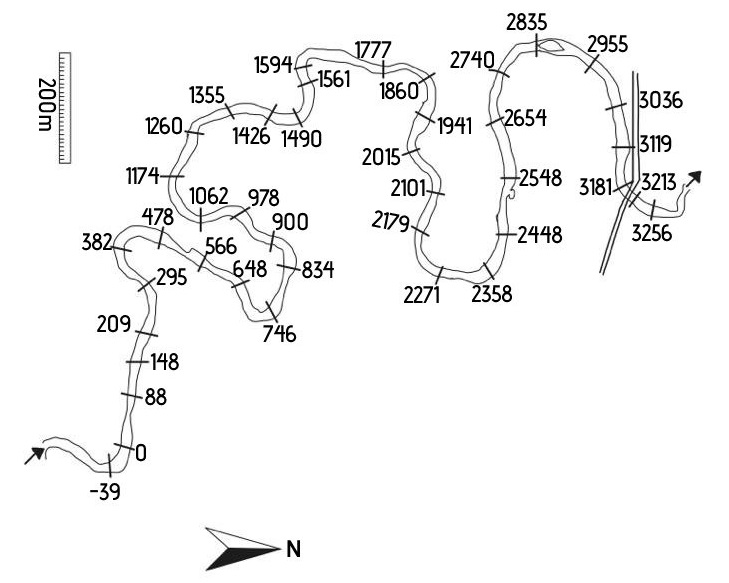
\includegraphics[width=0.7\textwidth]{ffjm2fig4.jpg}
\caption{Illustration of the 3.3~km stretch of the East Fork River
considered in the model, with markings of the data collection stations
used for boundary and initial conditions, recorded between May 17 and
June 17, 1977, as available in \cite{meade1979}. Image modified from
\cite{AYVAZ2013183}.}
\label{fig:east-fork-map}
\end{figure}
\FloatBarrier

Consider a grid with $n_{grid}$ points
$x_{min} = x_1 < \cdots < x_{n_{grid}} = x_{max}$. Collect the
$n_{grid}$ values $n_g(x_1), \ldots, n_g(x_{n_{grid}})$ into a parameter
vector $\xi \in \R^{n_{grid}}$, with $\xi_i := n_g(x_i)$ for
$i = 1, \ldots, n_{grid}$, kept notationally distinct from the spatial
coordinate $x$. In \cite{FortunatoMartinez2025}, this calibration problem
is posed as a constrained optimization problem, minimizing either the sum
of squared deviations of $\xi$ from a reference value $\bar n$ or the
sum of absolute deviations, subject to equality constraints requiring the
simulated elevations to match the $n_{obs}$ observations and a box
constraint $0 \le \xi_i \le n_g^{\max}$. It is solved there by a
Safeguarded Augmented Lagrangian method (Algorithm~2.1 of
\cite{FortunatoMartinez2025}), with BOBYQA or PRIMA handling the
subproblems.

The two applications differ mainly in how the underlying PDE is solved.
In this work we rely on a more stable PDE solver, which lets us compute
the derivative of the objective with respect to $\xi$ accurately. This is precisely what enables the gradient-based comparison carried out
below, namely BFGS and Algorithm~\ref{complexity}.1 against the
derivative-free BOBYQA. Figure~\ref{fig:solver-comparison} contrasts the
previous and the current solver on the same problem.

\begin{figure}[H]
	\centering
	\begin{minipage}{0.48\textwidth}
		\centering
		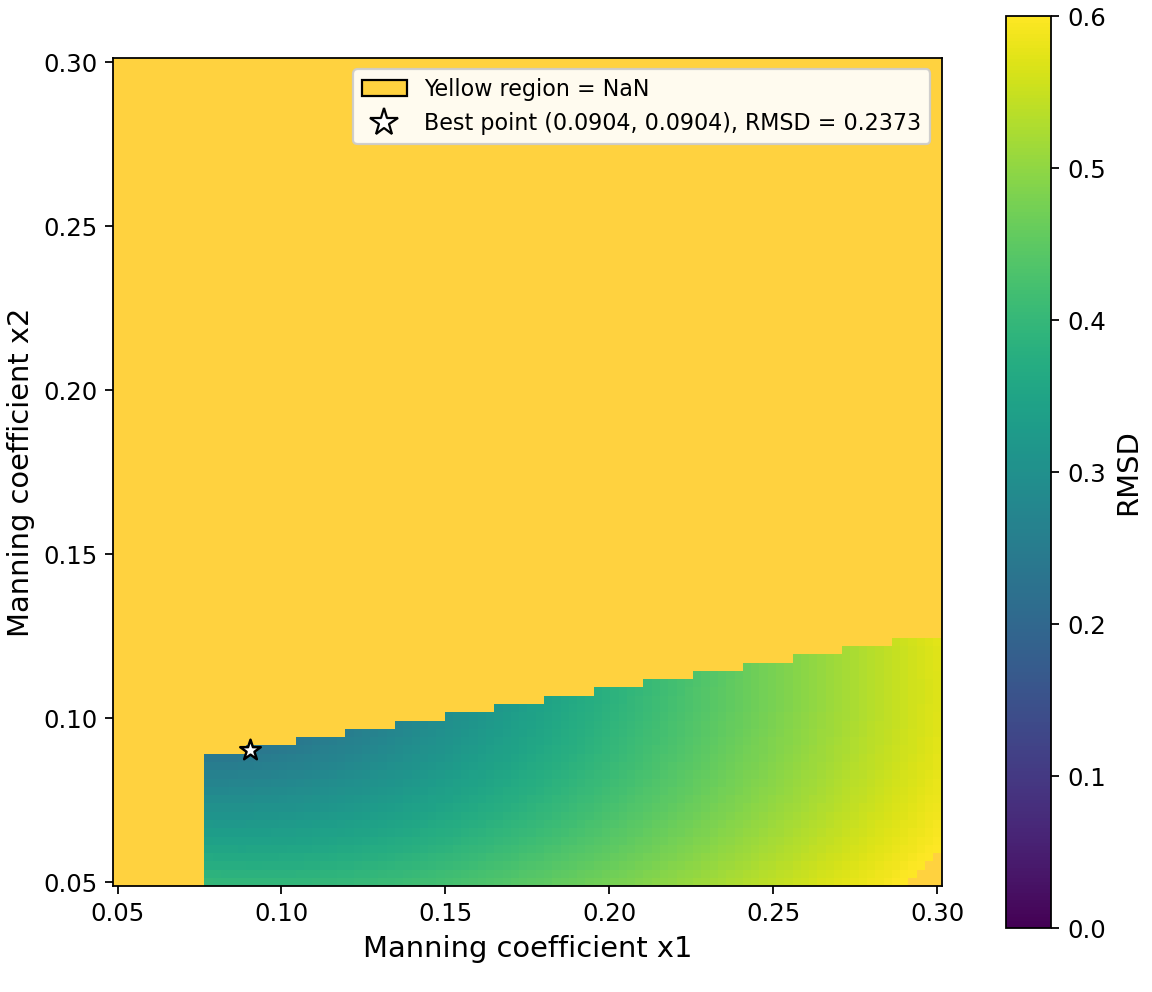
\includegraphics[width=\textwidth]{ffjm2fig5a.png}
	\end{minipage}
	\hfill
	\begin{minipage}{0.48\textwidth}
		\centering
		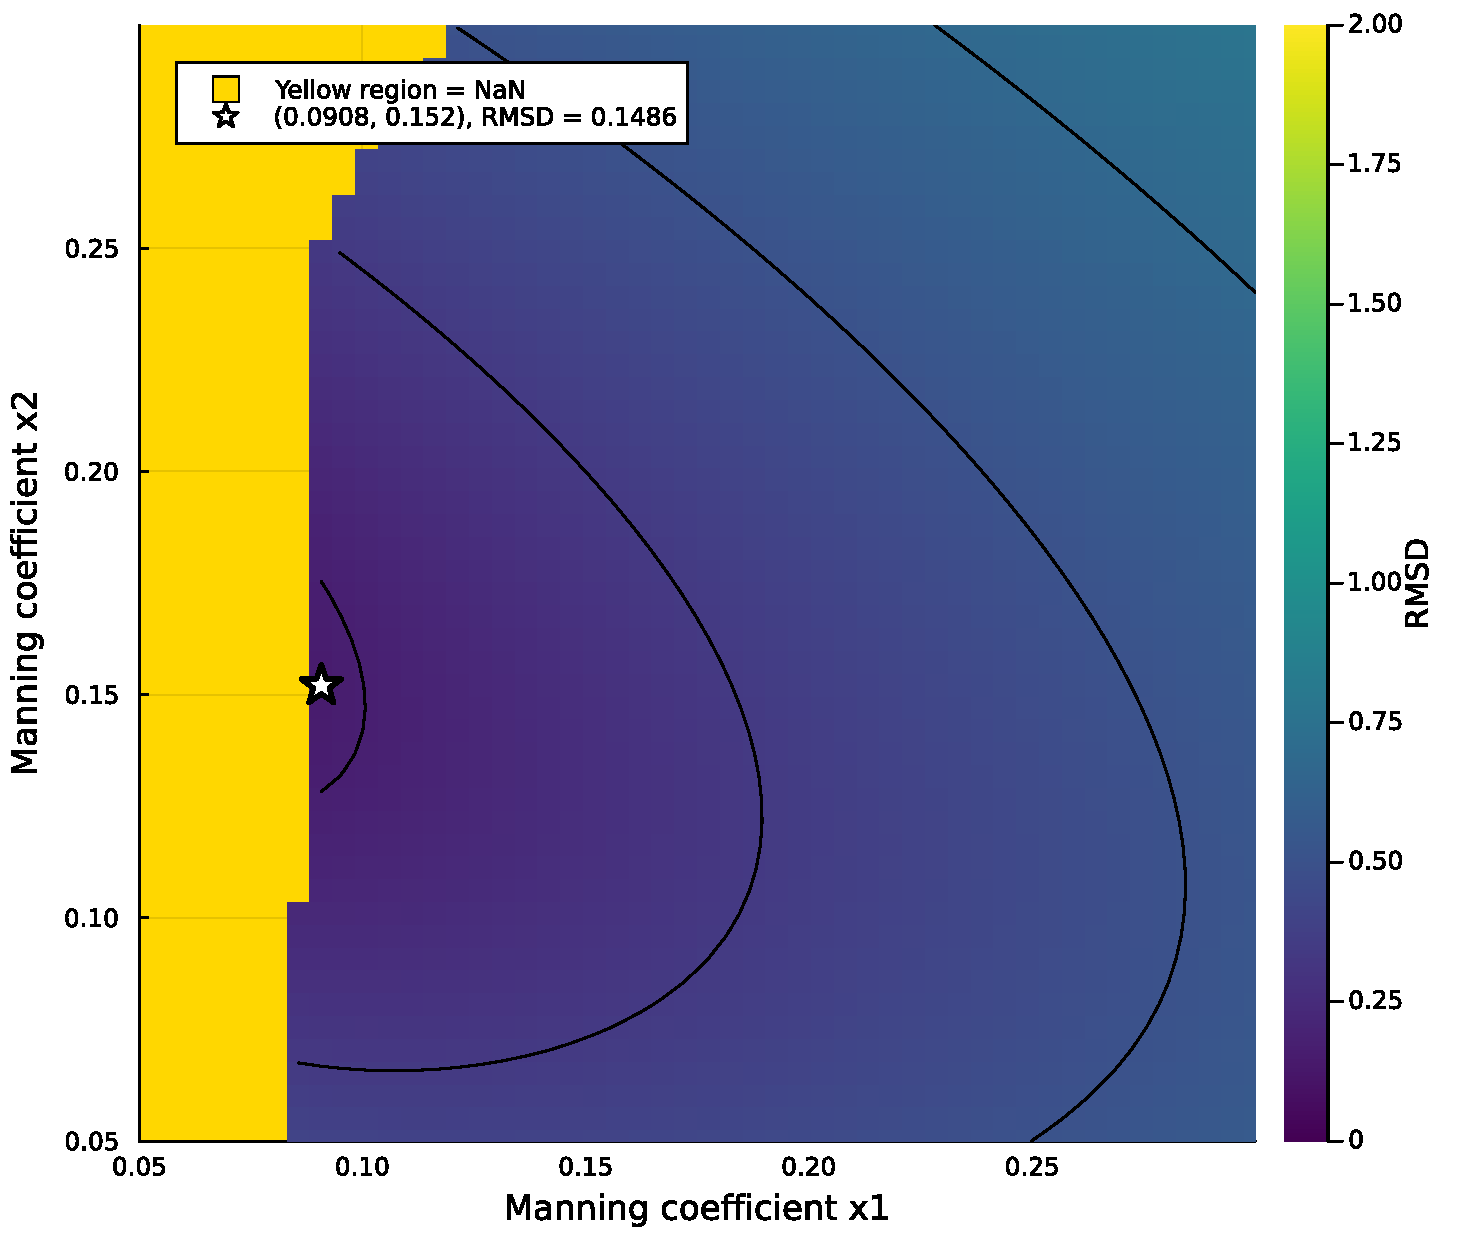
\includegraphics[width=\textwidth]{ffjm2fig5b.pdf}
	\end{minipage}
	\caption{Comparison between the previous (left) and the current (right) PDE solver.}
	\label{fig:solver-comparison}
\end{figure}
\FloatBarrier

For the comparison in this section, we adapt this into the unconstrained
nonlinear least-squares form used throughout this report, minimizing the
elevation mismatch directly instead of enforcing it as an equality
constraint. For $i = 1, \ldots, m$ (with $m = n_{obs}$), let
$z_i(\xi)$ denote the surface elevation the Saint-Venant solution
predicts, for parameter vector $\xi$, at the $i$-th observation's
location and time $(x_i, t_i)$, and let $z_{obs,i} = z_{obs}(x_i, t_i)$
be the corresponding observation. Define the residual components
$f_i(\xi) = z_i(\xi) - z_{obs,i}$, collect them into $F(\xi) =
(f_1(\xi), \ldots, f_m(\xi))^T$, and minimize
\[
f(\xi) = \frac12\|F(\xi)\|_2^2 = \frac12\sum_{i=1}^m f_i(\xi)^2.
\]
Calibrating $n_g$ against the observations is thus the nonlinear
least-squares problem of finding $\xi$ that minimizes $f(\xi)$
(ideally $F(\xi) = 0$, though the real data need not be exactly
consistent with the model).






\subsection{Experimental setup}
To calibrate $\xi$ against this residual, four benchmark scenarios
compare the same three solvers used throughout this report, namely BFGS
(backtracking, order 2), BOBYQA, and Algorithm~\ref{complexity}.1, applied
directly to $F(\xi)$ above where each solver stands in as the
whole optimizer, rather than as Algorithm~\ref{complexity}.1's internal
subproblem solver. Two scenarios use pregenerated data, where the
observations $z_{obs,i}$ are themselves generated by the model at a known
$\xi^\star$, so the true minimizer is known exactly. The other two use
the real observed data, where the true minimizer (if it exists) is
unknown. This real data is the one described previously, obtained from \cite{meade1979}. BFGS and BOBYQA
are both given the same box, $[0,0.5]^{n_{grid}}$,
and for the same reason, since a trial step that is too large
is likely to land in a forbidden region $P$ (in the terminology of
\cite{FortunatoMartinez2025}, this algorithm's own reference), a region
where the PDE simulation diverges and the residual is undefined, so
evaluating $F$ there is meaningless and wasted. BFGS enforces the box softly,
through an additive penalty term, $\frac12\|F(\xi)\|_2^2 +
\mathrm{penalty}(\xi)$, where $\mathrm{penalty}$ (weight $+\infty$)
evaluates to exactly $0$ whenever every coordinate of $\xi$ is feasible,
as is the case at every minimizer reported below. $F$ is still evaluated
everywhere, but the penalty discourages the line search from accepting
a step that reaches too far. BOBYQA instead enforces the same box as a
hard constraint, through NLopt's own bound support, so it minimizes
$\frac12\|F(\xi)\|_2^2$ unpenalized and NLopt never evaluates the
objective at a trial point outside the box in the first place.
Algorithm~\ref{complexity}.1
minimizes $f(\xi) = \frac12\|F(\xi)\|_2^2$ directly, with no box at all,
relying instead on its own $\sigma$-regularization to keep steps away
from that same region.

\subsubsection{Algorithmic settings}

All three solvers are implemented in Julia, version 1.10, and every
experiment reported in this section was run on a computer with a
5.2~GHz 12th Gen Intel(R) Core(TM) i9-12900K processor and 16~GB of
3200~MHz DDR4 RAM, running Linux Mint 21.1. They also share the same
evaluation budget, since each residual evaluation is a full transient
simulation of the Saint-Venant equations (BFGS and BOBYQA allowed at
most 1000 evaluations of the residual, Algorithm~\ref{complexity}.1 at
most 1000 outer iterations), and BFGS and Algorithm~\ref{complexity}.1
further share a gradient-norm convergence tolerance of $10^{-3}$; the
remaining settings differ per solver, as detailed below. The Status
column in Tables~\ref{tab:pregenerated-dim2}, \ref{tab:pregenerated-dim10},
\ref{tab:real-dim2}, and \ref{tab:real-dim10} reports each solver's own
termination code directly, \texttt{grad\_conv} (Algorithm~\ref{complexity}.1
or BFGS) and \texttt{Trust\_Region} (BOBYQA) marking a stopping
criterion that actually certifies stationarity, \texttt{reg\_stalled}
(Algorithm~\ref{complexity}.1's $\sigma$ stuck at its ceiling) and
\texttt{step\_conv} (BFGS's line search stuck at its minimum step)
marking a stall instead, and \texttt{maximum\_iterations},
\texttt{XTOL\_REACHED}, and \texttt{FTOL\_REACHED} marking the budget
above running out without either.

\begin{itemize}
	\item \textbf{BFGS}, the \texttt{BFGS} method from the
	\texttt{Optim.jl} package (version 2.0), together with the order-2
	backtracking line search from the \texttt{LineSearches.jl} package
	(version 7.7), the same combination used in
	Section~\ref{sec:mgh-problems}. Gradients are obtained by
	forward-mode automatic differentiation with the
	\texttt{ForwardDiff.jl} package (version 1.3), as discussed above.
	The line search gives up, reporting \texttt{step\_conv}, once its
	step length shrinks below $10^{-12}$, and the number of gradient
	evaluations is capped at 500.
	\item \textbf{BOBYQA}, the implementation provided by the
	\texttt{NLopt.jl} package (version 1.2). The trust region starts
	with radius $0.01$ and the search stops once it has shrunk to
	$10^{-6}$. The number of interpolation points and other internal
	settings are left at the package's own defaults.
	\item \textbf{Algorithm~\ref{complexity}.1}, our own Julia
	implementation, like the Saint-Venant solver itself. It uses the
	same regularization schedule described in Section~\ref{sec:mgh-problems},
	starting at $\sigma_0=1$ and growing by a factor of
	$\sigma_{grow}=10$ on every rejected step, with a floor of
	$\sigma_{\min}=10^{-8}$ and a ceiling of $\sigma_{\max}=10^{12}$
	kept purely for numerical stability.
\end{itemize}


\subsection{Results}

\begin{table}[htbp]
	\centering
	\caption{Pregenerated-data experiment, $n_{grid}=2$: $\xi^\star=(0.20,\,0.15)$,
		$\xi^0=(0.25,\,0.25)$.}
	\label{tab:pregenerated-dim2}
	\resizebox{\textwidth}{!}{%
		\begin{tabular}{l r r r r r r l}
			\toprule
			Method & RMSD & $f$ & $\|\nabla f\|$ & Func.\ evals & Grad.\ evals & Time (s) & Status \\
			\midrule
			BFGS (backtracking) & $7.47\times10^{-7}$ & $9.44\times10^{-11}$ & $1.48\times10^{-3}$ & 16 & 9 & 384.2 & \texttt{grad\_conv} \\
			BOBYQA & $4.61\times10^{-8}$ & $3.59\times10^{-13}$ & $6.94\times10^{-5}$ & 30 & 0 & 326.3 & \texttt{XTOL\_REACHED} \\
			Algorithm~\ref{complexity}.1 & $5.86\times10^{-11}$ & $5.80\times10^{-19}$ & $6.65\times10^{-8}$ & 10 & 5 & 158.0 & \texttt{grad\_conv} \\
			\bottomrule
		\end{tabular}
	}%
\end{table}
\FloatBarrier

\noindent
All three methods converge to essentially the exact reference
$\xi^\star=(0.20,0.15)$. Algorithm~\ref{complexity}.1 is the cheapest of the three by
every cost measure (fewest evaluations, least time) despite also reaching
the tightest gradient norm and RMSD.

\begin{figure}[H]
	\centering
	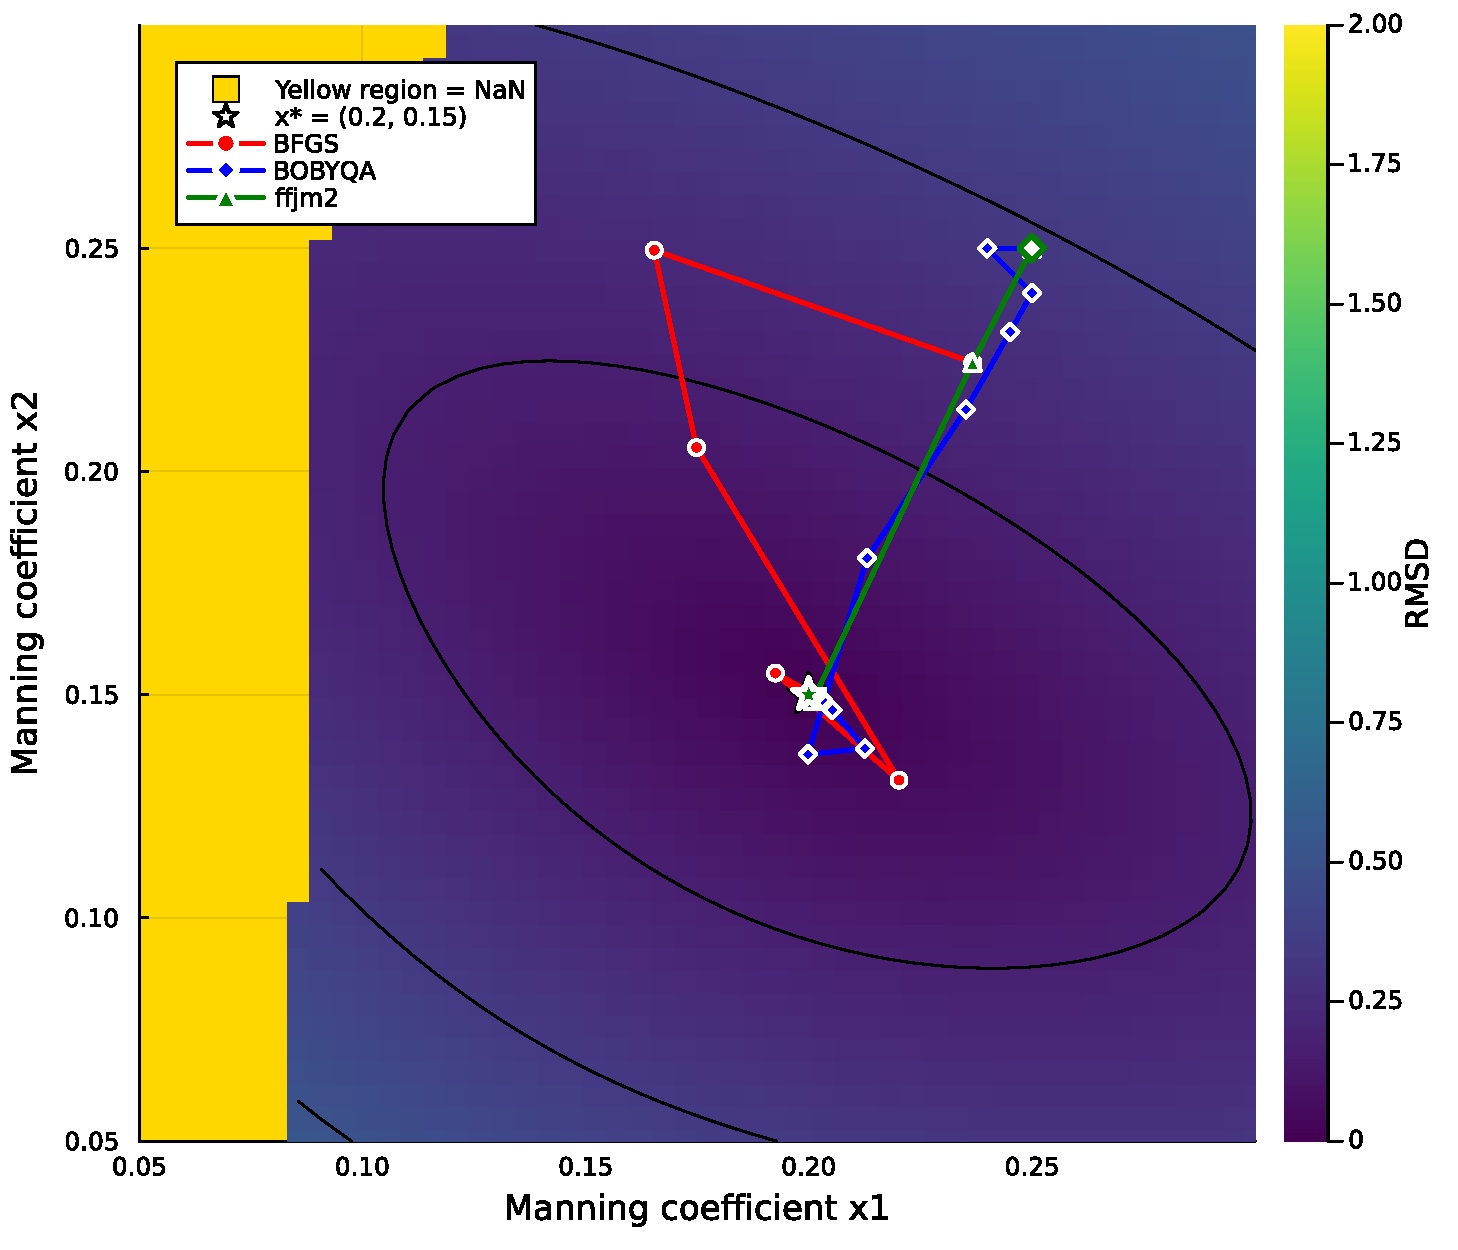
\includegraphics[width=0.8\linewidth]{ffjm2fig6.pdf}
	\caption{RMSD heatmap of the pregenerated-data experiment ($n_{grid}=2$) with the path of accepted iterates of each method overlaid: BFGS (red), BOBYQA (blue), and Algorithm~\ref{complexity}.1 (green), called \texttt{ffjm2}. The white diamond marks the shared starting point $\xi^0=(0.25,0.25)$. The star marks each method's final iterate.}
	\label{fig:performace_n_2_fake}
\end{figure}
\FloatBarrier



\begin{table}[htbp]
	\centering
	\caption{Pregenerated-data experiment, $n_{grid}=10$: decreasing profile $\xi^\star$
		from $0.20$ to $0.15$, $\xi^0=(0.25,\ldots,0.25)$.}
	\label{tab:pregenerated-dim10}
	\resizebox{\textwidth}{!}{%
		\begin{tabular}{l r r r r r r l}
			\toprule
			\FloatBarrier
			
			Method & RMSD & $f$ & $\|\nabla f\|$ & Func.\ evals & Grad.\ evals & Time (s) & Status \\
			\midrule
			BFGS (backtracking) & $2.00\times10^{-1}$ & $6.73\times10^{0}$ & $3.33\times10^{2}$ & 166 & 28 & 2453.6 & \texttt{step\_conv} \\
			BOBYQA & $3.68\times10^{-4}$ & $2.29\times10^{-5}$ & $1.26\times10^{-1}$ & 1000 & 0 & 12484.1 & \texttt{MAXEVAL\_REACHED} \\
			Algorithm~\ref{complexity}.1 & $4.38\times10^{-6}$ & $3.24\times10^{-9}$ & $1.02\times10^{-3}$ & 15 & 9 & 444.3 & \texttt{grad\_conv} \\
			\bottomrule
		\end{tabular}
	}%
\end{table}
\FloatBarrier


\begin{figure}[H]
	\centering
	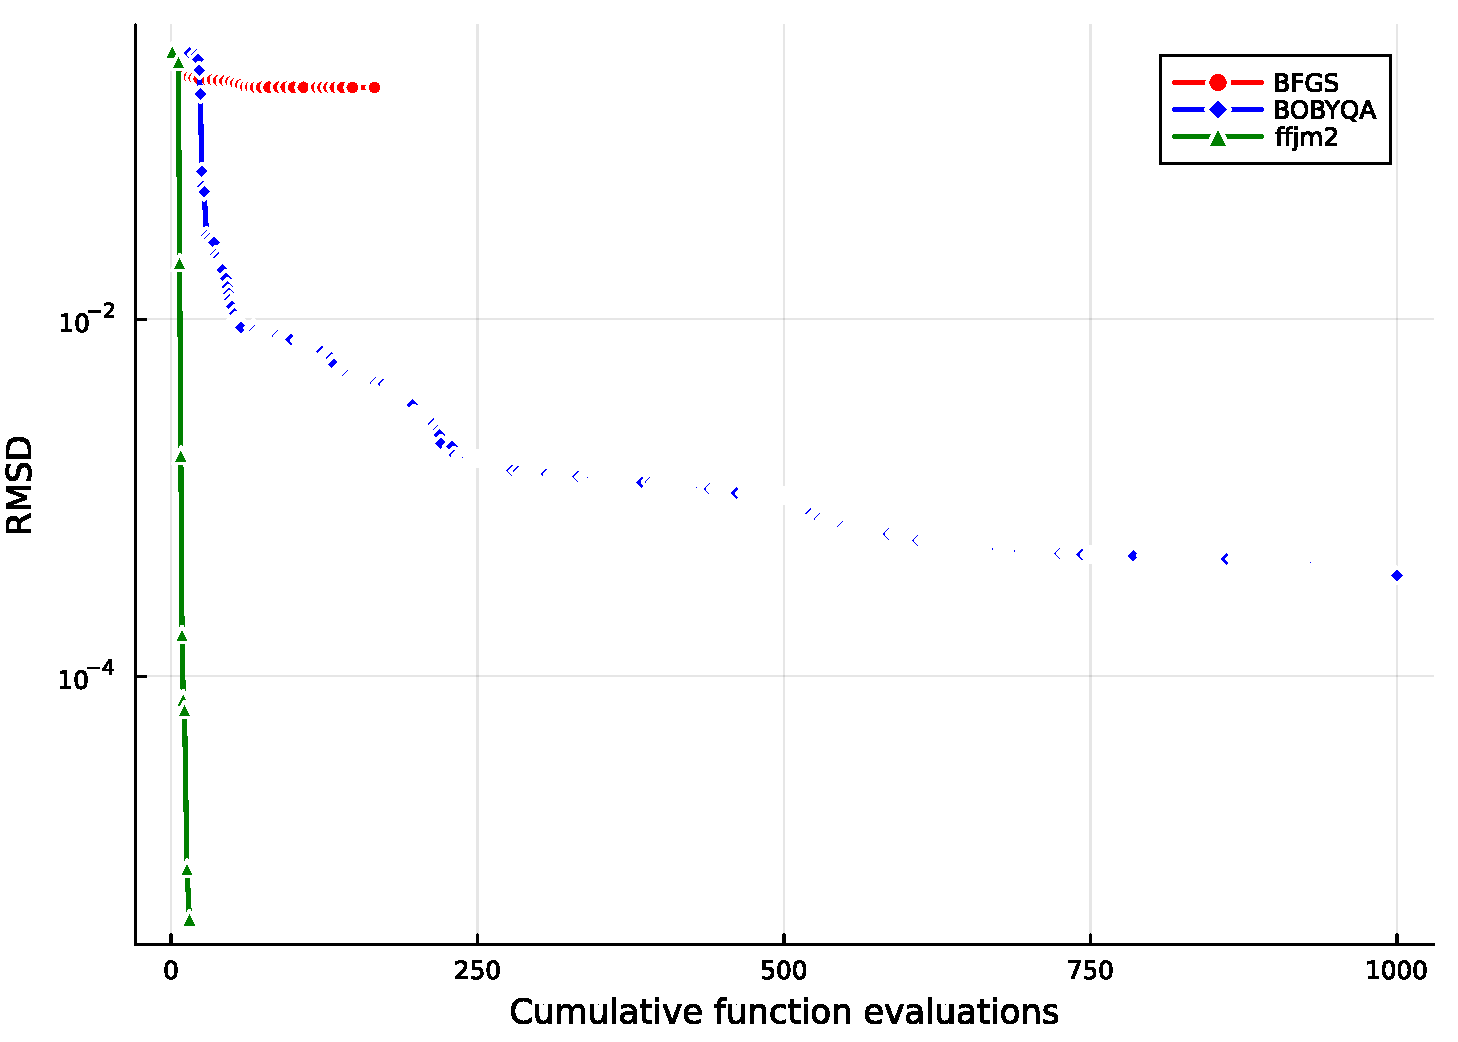
\includegraphics[width=0.75\linewidth]{ffjm2fig7.pdf}
	\caption{RMSD (log scale) against the cumulative number of function evaluations, for each method on the
		pregenerated-data experiment ($n_{grid}=10$): BFGS (red), BOBYQA (blue), and Algorithm~\ref{complexity}.1
		(green), called \texttt{ffjm2}. Each marker is one accepted iterate, in the order it was accepted.}
	\label{fig:rmsd-vs-evals-pregenerado-dim10}
\end{figure}
\FloatBarrier



\noindent
At $n_{grid}=10$ Algorithm~\ref{complexity}.1 is now the clear winner. It is
the only method that certifies a genuine stopping criterion
(\texttt{grad\_conv}, $\|\nabla f\|\approx1.02\times10^{-3}$), and it does
so at a small fraction of the cost of the other two ($15$ function and $9$
gradient evaluations, $444.3$s). BFGS's line search stalls
(\texttt{step\_conv}) with the worst RMSD and gradient norm of the three
($2.00\times10^{-1}$ and $\approx3.33\times10^2$, respectively).
BOBYQA gets much closer ($\text{RMSD}\approx3.68\times10^{-4}$, $\|\nabla
f\|\approx1.26\times10^{-1}$) but exhausts its evaluation budget
(\texttt{MAXEVAL\_REACHED}, $1000$ function evaluations) before
certifying convergence. At $n_{grid}=2$ all three methods converged, with
Algorithm~\ref{complexity}.1 already the cheapest of the three. 

\begin{table}[htbp]
	\centering
	\caption{Real data, $n_{grid}=2$: $\xi^0=(0.25,0.25)$.}
	\label{tab:real-dim2}
	\resizebox{\textwidth}{!}{%
		\begin{tabular}{l r r r r r r l}
			\toprule
			Method & RMSD & $f$ & $\|\nabla f\|$ & Func.\ evals & Grad.\ evals & Time (s) & Status \\
			\midrule
			BFGS (backtracking) & $2.10\times10^{-1}$ & $7.44\times10^{0}$ & $5.31\times10^{3}$ & 228 & 32 & 3191.3 & \texttt{step\_conv} \\
			BOBYQA & $1.42\times10^{-1}$ & $3.41\times10^{0}$ & $1.65\times10^{2}$ & 67 & 0 & 722.7 & \texttt{Trust\_Region} \\
			Algorithm~\ref{complexity}.1 & $1.42\times10^{-1}$ & $3.42\times10^{0}$ & $1.80\times10^{2}$ & 53 & 21 & 806.8 & \texttt{reg\_stalled} \\
			\bottomrule
		\end{tabular}
	}%
\end{table}
\FloatBarrier

\begin{figure}[H]
	\centering
	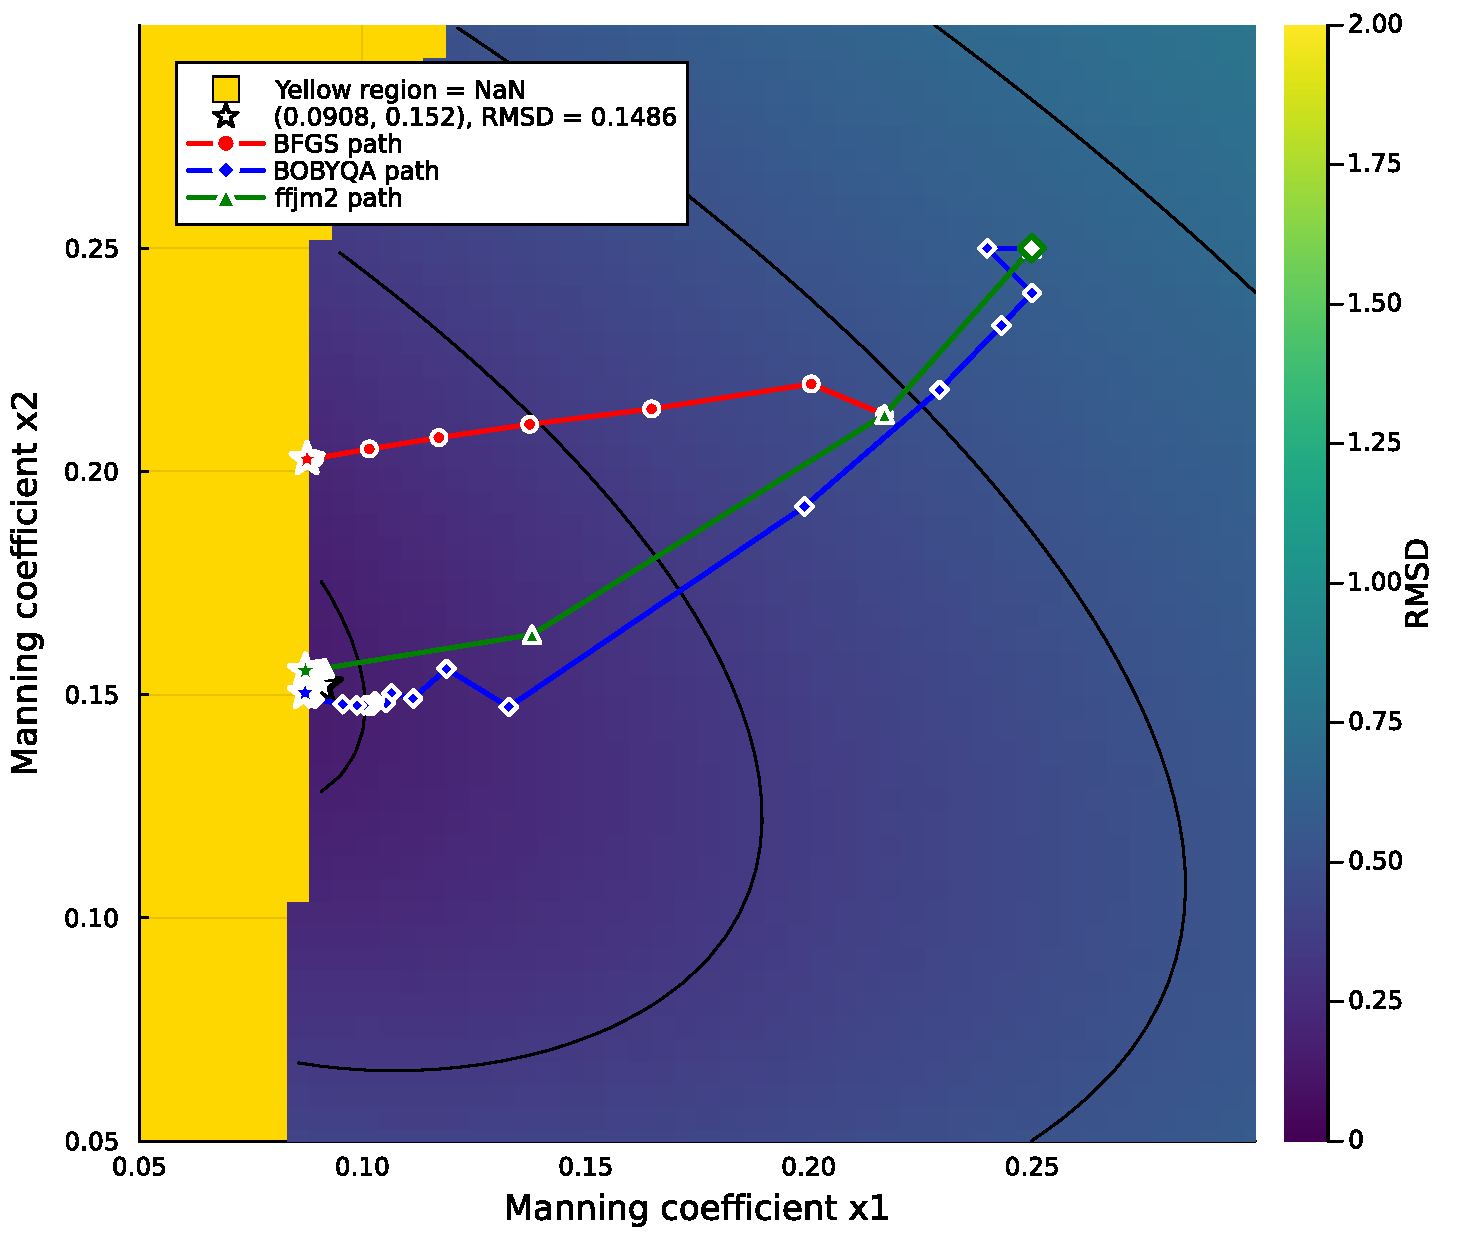
\includegraphics[width=0.8\linewidth]{ffjm2fig8.pdf}
	\caption{RMSD heatmap of the real-data experiment ($n_{grid}=2$) with the path of accepted iterates of each method overlaid: BFGS (red), BOBYQA (blue), and Algorithm~\ref{complexity}.1 (green), called \texttt{ffjm2}. The white diamond marks the shared starting point $\xi^0=(0.25,0.25)$, the star marks each method's final iterate.}
	\label{fig:performace_n_2_real}
\end{figure}
\FloatBarrier

\noindent
On real data, BFGS's line search stalls (\texttt{step\_conv}) before reaching a good point, with the worst
RMSD of the three ($2.10\times10^{-1}$) and a gradient norm still at
$\approx5.31\times10^3$. BOBYQA and Algorithm~\ref{complexity}.1 land on
essentially the same minimizer instead ($\xi\approx(0.087,\,0.155)$),
with matching RMSD ($1.42\times10^{-1}$) and $f$ $\approx3.41$--$3.42$. BOBYQA certifies its own
\texttt{Trust\_Region} criterion using fewer total evaluations and less wall-clock time
($722.7$s versus $806.8$s), while Algorithm~\ref{complexity}.1 again stalls
on $\sigma$ (\texttt{reg\_stalled}) just short of that same point.

\begin{table}[H]
	\centering
	\caption{Real data, $n_{grid}=10$: $\xi^0=(0.25,\ldots,0.25)$.}
	\label{tab:real-dim10}
	\resizebox{\textwidth}{!}{%
		\begin{tabular}{l r r r r r r l}
			\toprule
			Method & RMSD & $f$ & $\|\nabla f\|$ & Func.\ evals & Grad.\ evals & Time (s) & Status \\
			\midrule
			BFGS (backtracking) & $5.15\times10^{-2}$ & $4.49\times10^{-1}$ & $1.26\times10^{2}$ & 221 & 61 & 6253.5 & \texttt{step\_conv} \\
			BOBYQA & $4.68\times10^{-2}$ & $3.70\times10^{-1}$ & $8.67\times10^{-1}$ & 772 & 0 & 9120.5 & \texttt{Trust\_Region} \\
			Algorithm~\ref{complexity}.1 & $4.58\times10^{-2}$ & $3.54\times10^{-1}$ & $7.08\times10^{-1}$ & 60 & 24 & 1258.2 & \texttt{reg\_stalled} \\
			\bottomrule
		\end{tabular}
	}%
\end{table}
\FloatBarrier


\begin{figure}[H]
	\centering
	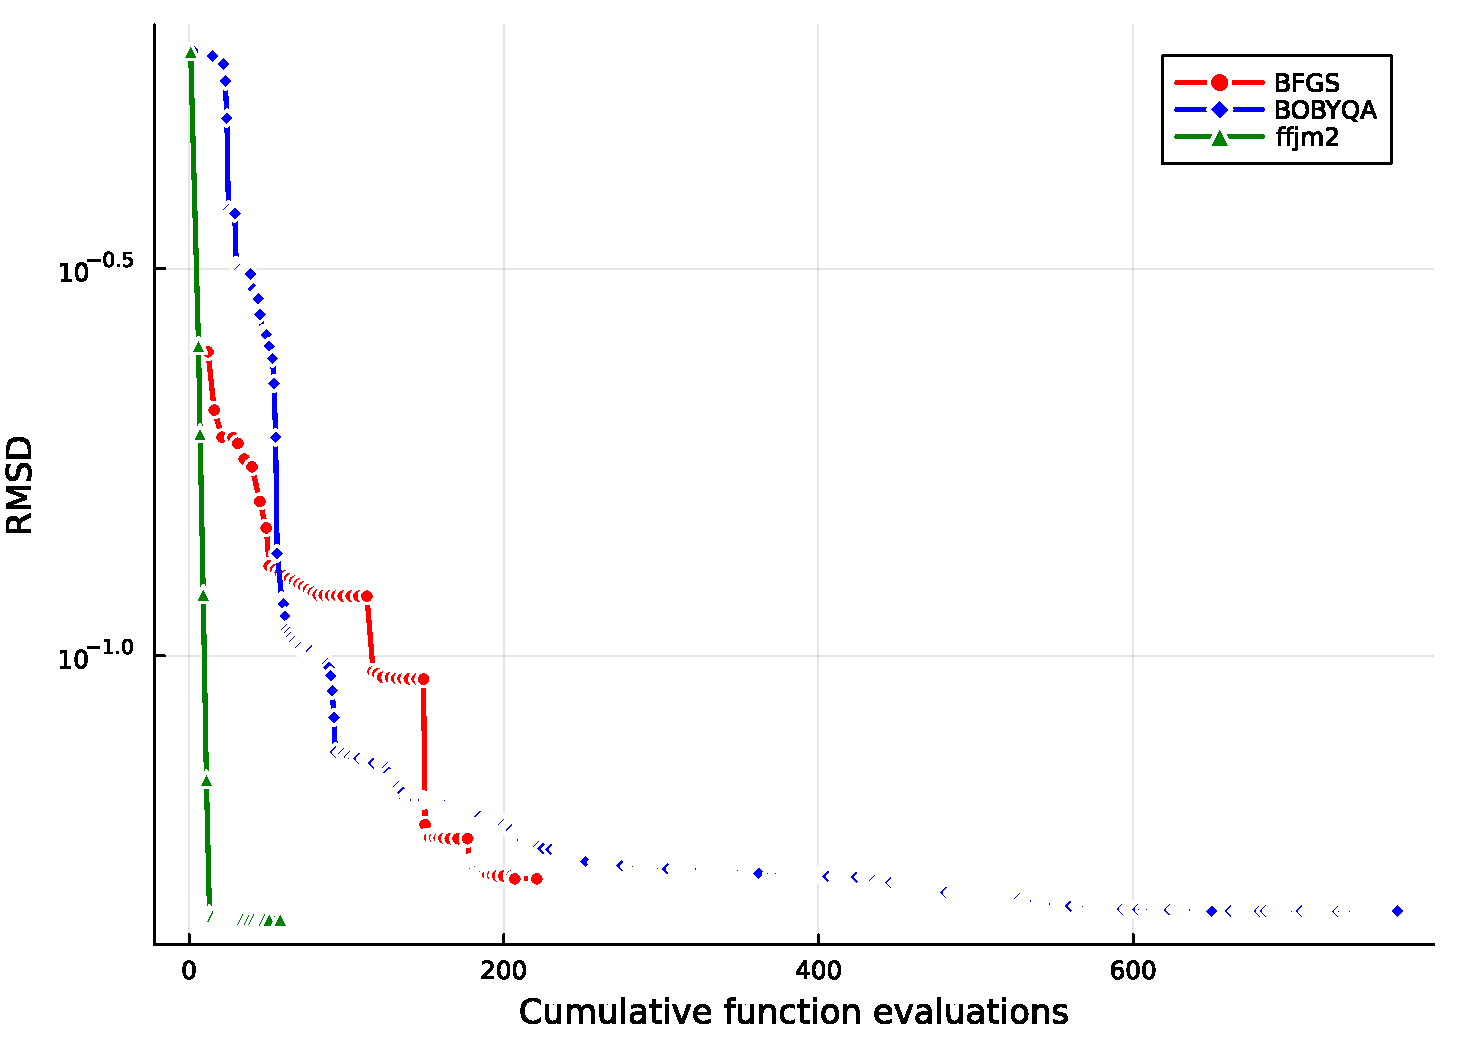
\includegraphics[width=0.8\linewidth]{ffjm2fig9.pdf}
	\caption{RMSD (log scale) against the cumulative number of function evaluations, for each method on the
		real-data experiment ($n_{grid}=10$): BFGS (red), BOBYQA (blue), and Algorithm~\ref{complexity}.1
		(green), called \texttt{ffjm2}. Each marker is one accepted iterate, in the order it was accepted.}
	\label{fig:rmsd-vs-evals-real-dim10}
\end{figure}
\FloatBarrier

\noindent
This remains the hardest of the four scenarios: none of the three
methods certifies a genuine stopping criterion. BFGS's line search
stalls (\texttt{step\_conv}) with the
largest gradient norm of the three ($1.26\times10^2$) and the
worst RMSD ($5.15\times10^{-2}$). BOBYQA certifies its own
\texttt{Trust\_Region} criterion, using $772$ evaluations and
$2.5$h to reach RMSD near to $4.68\times10^{-2}$. Algorithm~\ref{complexity}.1's
regularization parameter again hits its ceiling
(\texttt{reg\_stalled}), but this time it is the best of the three by
every measure: the smallest gradient norm ($7.08\times10^{-1}$,
even below BOBYQA's), the lowest RMSD ($4.58\times10^{-2}$), and by far
the lowest cost ($60$ residual and $24$ Jacobian evaluations,
$21$min, against BOBYQA's $772$ evaluations and BFGS's
$282$). This is the opposite of the $n_{grid}=10$ pregenerated-data
scenario (Table~\ref{tab:pregenerated-dim10}), where the same stall left
Algorithm~\ref{complexity}.1 the worst of the three, here it is both the cheapest
and the most accurate. All three still land on different minimizers with
comparable RMSD ($4.6$--$5.2\times10^{-2}$), and none certifies
first-order optimality.



\section{Conclusion} \label{conclusions}

This paper addresses two difficulties that often arise together in
optimization problems. Evaluating the objective function, and
especially its gradient, may be computationally expensive, so an
optimization algorithm must make the most of every such evaluation. At
the same time, the domain of the objective function may be restricted
by hidden constraints, unknown in advance and not always expressible
via equations or inequalities, since the underlying simulation may
simply blow up in certain regions, leaving the residual undefined
there. Parameter estimation for models governed by partial
differential equations is one important class of problems where both
difficulties arise, and the focus of this paper, though the
difficulties themselves are more general and arise whenever
calibrating any expensive-to-solve system of equations.

Sections~\ref{forbid} and~\ref{opfor} handle the first difficulty on
its own, for a general smooth unconstrained objective. Algorithm~\ref{opfor}.1
adapts a classical line-search scheme by treating a forbidden trial
point exactly as a rejected one, without ever using a function value
that does not exist. Every iteration is well defined
(Lemma~\ref{opfor}.1), and every limit point of the generated sequence
is either a forbidden point or a stationary point
(Theorem~\ref{opfor}.1). Notably, this guarantee requires no
Lipschitz or H\"older condition on $\nabla f$. Prior treatments of
such hidden constraints are largely derivative-free, such as the
extreme-barrier rule used in Mesh Adaptive Direct Search
\cite{mads,audetdennis,bcls,LeDigabelWild2024,rz}, some of them built
around a line-search structure \cite{fllr,GrattonVicente2014}, and
come with little accompanying convergence theory. Algorithm~\ref{opfor}.1
extends the same idea, of treating a forbidden trial point as a plain
rejected one within a backtracking line search, to the gradient-based
case, with an explicit convergence guarantee that fills that
theoretical gap.

Section~\ref{complexity} turns to the second difficulty, proposing
Algorithm~\ref{complexity}.1. At each
iteration it minimizes a quartic model built from per-residual
quasi-Newton Hessians, regularized by a parameter $\sigma$. Unlike
Algorithm~\ref{opfor}.1, it requires no line search at all. A rejected
trial step only increases $\sigma$ and re-solves the resulting
subproblem, rather than rescaling a fixed direction along a ray. It is
also independent of the value assigned to a forbidden point, since
feasibility is checked directly, before that value could ever enter a
comparison, so the same guarantees hold whether such a point is
represented by $+\infty$ or by an arbitrarily large finite penalty.
Under a Lipschitz-type condition on the residual gradients
(Assumption~\ref{complexity}.1), Algorithm~\ref{complexity}.1 is well
defined (Lemma~\ref{complexity}.1), drives $\|s^k\|\to0$
(Theorem~\ref{complexity}.2), and reaches
$\|\nabla f(x^k)\|\le\varepsilon$ in at most $O(\varepsilon^{-2})$
iterations whenever $x^k$ stays a fixed distance away from the
forbidden set (Theorems~\ref{complexity}.3--\ref{complexity}.4 and
Corollary~\ref{complexity}.1).

Section~\ref{sec:degeneracy} identifies and resolves a degeneracy
specific to this scheme. At the very first iteration ($k=0$) no
quasi-Newton curvature has yet been observed, so the quartic model
collapses to a damped Gauss--Newton quadratic. We show that its
minimizer is a descent direction for every $\sigma>0$
(Lemma~\ref{sec:closedform}.1) and becomes asymptotically parallel to
$-\nabla f(x^0)$ as $\sigma\to\infty$ (Proposition~\ref{sec:closedform}.2),
so the regularization ladder already behaves like a backtracking line
search along $-\nabla f(x^0)$ once $\sigma$ is large enough, with no
separate safeguard required. This matters in practice because $\sigma$
is never reset between outer iterations, only carried over up to a
constant factor. Since no curvature information is yet available at
$k=0$, an unnecessarily large $\sigma$ forced at that very first
iteration would persist into later iterations and dampen them more
than necessary.


Section~\ref{sec:computational-tests} calibrates Algorithm~\ref{complexity}.1
on the 34 MGH sum-of-squares problems~\cite{MoreGarbowHillstrom1981},
settling on the PSB Hessian update and an exact Newton step for the
quartic subproblem, and on an order-2 backtracking line search for the
BFGS baseline it is compared against. Over all 34 problems, the two
reach statistically indistinguishable final objective values
(Mann-Whitney test), while Algorithm~\ref{complexity}.1 is
significantly cheaper, the better or tied method on about 80\% of the
problems.

Section~\ref{cap:coeficient_estimation} takes Algorithm~\ref{complexity}.1, BFGS, and
the derivative-free BOBYQA to a real engineering problem, calibrating
the spatially varying Manning coefficient of the Saint-Venant
equations from elevation observations, across four scenarios
(synthetic and real data, at dimension 2 and 10). Algorithm~\ref{complexity}.1 is the
cheapest and most accurate of the three in three of the four
scenarios. The exception is the synthetic dimension-10 case, where its
regularization parameter $\sigma$ hits its ceiling and it becomes the
worst of the three instead. The same stall reappears on real data at
dimension 10, the hardest of the four scenarios, but there it costs
nothing: Algorithm~\ref{complexity}.1 is again the cheapest and most accurate.

Taken together, these results show that Algorithm~\ref{complexity}.1
is efficient and competitive at solving both classical test problems
and real engineering problems, offering a practical alternative to
BFGS and BOBYQA for expensive sum-of-squares problems defined on a
domain with forbidden regions, and typically the cheapest of the three
whenever it converges.

A weakness of the method is that its surrogate is a quartic model, so
global optimality of the subproblem itself cannot be guaranteed, only
an approximate global solution obtained by multistart. However, note
that global solution of the subproblem is not needed at all in the
definition of the algorithm. Moreover, once
this model no longer represents the objective function well, it must
be reset entirely rather than merely updated, which can be a problem
when the minimization starts far from a solution of a strongly
non-quadratic objective.

For future work, we intend to better characterize when the model
stops representing the objective function well. Currently this is
judged in aggregate, through the ratio $\rho_k$ between actual and
predicted reduction in $f$, which triggers a reset of every $H_i$ at
once. Examining each residual $f_i$ individually seems like a
promising alternative, and could guide decisions to further improve
the proposed algorithm. We also intend to apply the algorithm to
larger and more complex problems, where its efficiency advantage may
become even more evident.




       
 
               
%
%\section{Numerical Experiments} \label{numerical}
%
%  Our experiments were run using a computer with a 5.2 GHz 12th Gen Intel(R) Core(TM) i9-
%12900K processor and 16GB 3200 MHz DDR4 RAM memory, running Linux Mint 21.1. The code
%was compiled by the GFortran compiler of GCC (version 11.3.0) with the -O3 optimization directive
%enabled.          
% 
%
%Por Taylor, dado $a \in \R^n$, temos que 
%\[
%f_i(x) = f_i(a) + \nabla f_i(a)^T (x - a) + \half (x-a)^T \nabla^2 f_i(a) (x - a) + O(\|x-a\|^3).
%\]
%Portanto,
% \[
%f_i(x)^2 = [f_i(a) + \nabla f_i(a)^T (x - a) + \half (x-a)^T \nabla^2 f_i(a) (x - a)]^2  
%\]
%\[
%+ 2[f_i(a)  + 
% \nabla f_i(a)^T(x-a) +  \half (x-a)^T \nabla^2 f_i(a) (x - a)]^2]  O(\|x-a\|^3) + O(\|x-a\|^6). 
%\]  
%
%Logo,
%\begin{equation} \label{apro}
%f(x) = \sum_{i=1}^m   [f_i(a) + \nabla f_i(a)^T (x - a) + \half (x-a)^T \nabla^2 f_i(a) (x - a)]^2  + f(a)   O(\|x-a\|^3). 
%\end{equation}
%
%Esta fórmula induz de idea de minimizar, em cada iteração, a função
%    $\sum_{i=1}^m   [f_i(a) + \nabla f_i(a)^T (x - a) + \half (x-a)^T \nabla^2 f_i(a) (x - a)]^2$. Mas isto é impraticável
%  devido ao custo de $\nabla^2 f_i$.
%
%Entretanto, podemos adotar a ideia de aproximar, via fórmulas quase-Newton, essas Hessianas. Isso leva à proposta de minimizar
% em cada iteração:
%\begin{equation} \label{thesu}
%\mbox{ Minimizar }\sum_{i=1}^m   [f_i(a) + \nabla f_i(a)^T (x - a) + \half (x-a)^T H_i(a) (x - a)]^2.
%\end{equation}
%sujeita a uma região de confiança ou acrescentada de uma regularização.
%
%(\ref{thesu}) é a minimização de uma quártica, o que normalmente não é aconselhável. Mas no contexto de funções muito
%caras, esta ideia pode ser viável. Logo, para minimizar globalmente (\ref{thesu}) não poupariamos esforços.
%
%Há muitas fórmulas quase-Newton. Por exemplo, as fórmulas BFGS e SR1, que são as seguintes:
%\begin{equation} \label{bfgs}
%H_+ = H + y y^T/s^T y - (H s s^T H)/(s^T H s)
%\end{equation}
%e
%\begin{equation}\label{sr1}
%H_+ = H + (y - Hs)(y - Hs)^T/(y- Hs)^T s.
%\end{equation}
%
%
% Estas fórmulas são as que vão definir a direção $d^k$ no Algoritmo \ref{opfor}.1, da seguinte maneira.
%
%\begin{enumerate}
%
%\item Inicializar $H_i = 0$ para todo $i = 1, \ldots, m$.
%
%\item Se $k = 0$, $d^k = -\nabla f(x^k)$.
%
%\item Se $k > 0$ definir $s \leftarrow x^k - x^{k-1}$, Para cada $i=1,\ldots,m$ calcular $y = \nabla f_i(x^k) - \nabla f_i(x^{k-1})$.  
% Para cada $i=1,\ldots,m$  calcular $H_+$ usando (\ref{bfgs}) ou (\ref{sr1}). Definir $H \leftarrow H_+$. Resolver, globalmente,  
% (\ref{thesu}) com $a = x^k$, obtendo $x$. Definir $d^k = x - x^k$. Verificar as condições (\ref{conds}). Se não se verificam,
%  substituír $d^k$ pela direção de $-\nabla f(x^k)$. Espero que se verifiquem sempre, em caso contrário tanto trabalho foi jogado
%  no lixo.  
%
%\end{enumerate}
%
% 
%
%
%\section{Experiments Concerning Parameter Estimation of river-Flow Modelling} \label{river}
%
%\section{Conclusions} \label{conclusions}


    
\begin{thebibliography}{9999}

 

\bibitem{Agresta2021} A. Agresta, M. Baioletti, C. Biscarini, and A. Milani, Evolutionary Algorithms
 for Roughness Coefficient Estimation in River Flow Analyses, in {\it Applications of Evolutionary
 Computation (EvoApplications 2021)}, Lecture Notes in Computer Science 12694, Springer,
 pp.~795--811, 2021.
%
%

\bibitem{mads} Ch. Audet and J. E. Dennis Jr. {Mesh adaptive direct search algorithms 
for constrained optimization,} {\it SIAM Journal on Optimization}~17, pp. 188--217, 2006.
%

\bibitem{audetdennis} Ch. Audet, J. E. Dennis Jr., 
and S. Le Digabel, {Globalization strategies for Mesh
 Adaptive Direct Search},  {\it Computational Optimization and Applications} 46,
 pp. 193--215, 2010.
%

 \bibitem{AYVAZ2013183} M. T. Ayvaz, A linked simulation–optimization model for simultaneously estimating 
the Manning’s surface roughness values and their parameter structures in shallow water flows, {\it Journal of Hydrology} 500, pp.~183--199, 2013.  

   \bibitem{bcgmr} E. G. Birgin, M. R. Correa, V. A. González-López, J. M.  Mart\'{\i}nez, and D. S. Rodrigues,
 Randomly supported variation of deterministic models and its application to one-dimensional shallow
water flows, {\it Journal of Hydraulic Engineering}~150(5): 04024026, 2024.

\bibitem{BirginMartinez2022} E. G. Birgin and J. M. Mart\'{\i}nez, Accelerated derivative-free
 nonlinear least-squares applied to the estimation of Manning coefficients, {\it Computational
 Optimization and Applications} 81, pp.~689--715, 2022.

%\bibitem{bfm} E. G. Birgin, C. Floudas, and J. M. Mart\'{\i}nez.
% {   Global minimization using an Augmented Lagrangian method with
%variable lower-level constraints }, {\it Mathematical Programming} 
%   125, pp. 139--162, 2010.    

 \bibitem{bmbook} E. G. Birgin and J. M. Mart\'{\i}nez,
  \textit{Practical Augmented Lagrangian Methods for Constrained
    Optimization}, Society for Industrial and Applied Mathematics,
  Philadelphia, 2014.

\bibitem{bcls} A. Brilli, A. L. Cust\'odio, G. Liuzzi, and E. J. Silva,
   Nonlinear derivative-free constrained optimization with a penalty-interior point method and
   direct search, {\it Numerical Algorithms}, 2026, https://doi.org/10.1007/s11075-026-02360-5.

\bibitem{Broyden1970} C. G. Broyden, The convergence of a class of double-rank minimization
 algorithms 2. The new algorithm, {\it IMA Journal of Applied Mathematics} 6, pp.~222--231, 1970.

\bibitem{CartisGouldToint2011a} C. Cartis, N. I. M. Gould, and Ph. L. Toint, Adaptive cubic regularisation
 methods for unconstrained optimization. Part I: motivation, convergence and numerical results,
 {\it Mathematical Programming} 127(2), pp.~245--295, 2011.
%

\bibitem{CartisGouldToint2011b} C. Cartis, N. I. M. Gould, and Ph. L. Toint, Adaptive cubic regularisation
 methods for unconstrained optimization. Part II: worst-case function- and derivative-evaluation
 complexity, {\it Mathematical Programming} 130(2), pp.~295--319, 2011.

\bibitem{castro} O. Castro-Orgaz and W. H. Hager, {\it Shallow Water Hydraulics}, Springer, 2019. 

\bibitem{csvbook} A. R. Conn, K. Scheinberg, 
 and L. N. Vicente. \textit{Introduction to Derivative-Free Optimization}, MPS-SIAM Series on Optimization, SIAM, Philadelphia, 2009.

%\bibitem{cgr} A. L. Custódio, R. Garmanjani, and M. Raydan, Derivative-free 
%separable quadratic modeling and cubic regularization for unconstrained optimization, {\it 4OR } 22, pp. 121 - 144, 2024.

%\bibitem{custodio} A. L. Cust\'odio and L. N. Vicente, {Using sampling and simplex derivatives 
%in pattern search methods,} {\it SIAM Journal on Optimization}~18, pp. 537--555, 2007.

\bibitem{DennisWolkowicz1993}
J. E. Dennis, Jr. and H. Wolkowicz, \emph{Sizing and least-change secant
	methods}, SIAM J. Numer. Anal., 30 (1993), pp.~1291--1314.

% \bibitem{dmp} M. A. Diniz-Ehrhardt, J. M. Mart\'{\i}nez, and 
%  L. G. Pedroso,  Derivative-free  methods for nonlinear programming
% with general lower-level constraints, 
% {\it Computational \& Applied Mathematics} 30, pp.~19--52, 2011.      

\bibitem{DolanMore2002}
E. D. Dolan and J. J. Mor\'e, \emph{Benchmarking optimization software
	with performance profiles}, Math. Program., 91 (2002), pp.~201--213.

\bibitem{fllr} G. Fasano, G. Liuzzi, S. Lucidi, and F. Rinaldi, A line search derivative-free approach for nonsmooth constrained
 optimization, {\it SIAM Journal on Optimization } 24, pp.~959--992, 2014.

\bibitem{Ferreira2017} D. M. Ferreira, C. V. S. Fernandes, and J. Gomes, Verification of Saint-Venant equations solution based 
on the Lax diffusive method for flow routing in natural channels, {\it Revista Brasileira de Recursos Hídricos}, vol.~22, 2017.
             https://doi.org/10.1590/2318-0331.011716104 

\bibitem{Fletcher1970} R. Fletcher, A new approach to variable metric algorithms, {\it The
 Computer Journal} 13, pp.~317--322, 1970.

\bibitem{FortunatoMartinez2025}
F. A. Fortunato and J. M. Mart\'inez, \emph{KKT-free constrained
	optimization and application to river-flow modelling}, {\it Optimization
	Methods and Software}, pp.~1--32, 2026, https://doi.org/10.1080/10556788.2026.2682934.

\bibitem{gllt} D. Ge, J. Liu, T. Liu, and J. Tan, 
 1053: SOLNP+: A Derivative-Free Solver for Constrained Nonlinear Optimization, 
   {\it ACM Transactions on Mathematical Software} 50(4),  DOI:10.1145/3699956, 2024.         

\bibitem{Goldfarb1970} D. Goldfarb, A family of variable-metric methods derived by variational
 means, {\it Mathematics of Computation} 24, pp.~23--26, 1970.

\bibitem{GrattonVicente2014} S. Gratton and L. N. Vicente, A merit function approach for direct
 search, {\it SIAM Journal on Optimization} 24(4), pp.~1980--1998, 2014.

%\bibitem{hestenes} M. R. Hestenes, {Multiplier and gradient methods,} {\it Journal of Optimization
% Theory and Applications}~4, pp. 303--320, 1969.

\bibitem{Hosseiny2022} H. Hosseiny, Implementation of heuristic search algorithms in the calibration
 of a river hydraulic model, {\it Environmental Modelling \& Software} 157, 105537, 2022.

\bibitem{Kang2024} H. Kang, Y. Kim, H. An, J. Byun, and J. Noh, Estimation of river discharge using
 Monte Carlo simulations and a 1D hydraulic model based on the artificial multi-segmented rating
 curves at the confluence of two rivers, {\it Environmental Research Communications} 6(2), 025012, 2024.

\bibitem{LeDigabelWild2024} S. Le Digabel and S. M. Wild, A taxonomy of constraints in black-box
 simulation-based optimization, {\it Optimization and Engineering} 25, pp.~1125--1143, 2024.

\bibitem{leveque} R. J. LeVeque, \textit{Numerical Methods for
Conservation Laws}, Lectures in Mathematics, ETH Z\"urich,
Birk\"auser, 1992.

\bibitem{MannWhitney1947} H. B. Mann and D. R. Whitney, On a test of whether one of two random
variables is stochastically larger than the other, {\it Annals of Mathematical Statistics} 18(1), pp.~50--60, 1947.

\bibitem{Martinez2024} J. M. Mart\'inez, Levenberg-Marquardt revisited and parameter tuning of
river regression models, {\it Computational and Applied Mathematics} 43, 14, 2024,
https://doi.org/10.1007/s40314-023-02535-z.

\bibitem{meade1979} R. H. Meade, R. M. Myrick, and W. W. Emmett, Field data describing the movement and storage of sediment
in the East Fork River, Wyoming, Part II, {\it USGS Open-File}, 1979.

 \bibitem{Mogensen2018}
 P. K. Mogensen and A. N. Riseth, \emph{Optim: A mathematical optimization
 	package for Julia}, J. Open Source Software, 3 (2018), p.~615.

 \bibitem{MoreGarbowHillstrom1981}
J. J. Mor\'e, B. S. Garbow, and K. E. Hillstrom, \emph{Testing
	unconstrained optimization software}, ACM Trans. Math. Software, 7 (1981),
pp.~17--41.

\bibitem{Nguyen2016} V. T. Nguyen, D. Georges, and G. Besan\c{c}on, State and parameter estimation
 in 1-D hyperbolic PDEs based on an adjoint method, {\it Automatica} 67, pp.~185--191, 2016.

\bibitem{NocedalWright2006} J. Nocedal and S. J. Wright, \textit{Numerical Optimization}, 2nd
 edition, Springer Series in Operations Research and Financial Engineering, Springer, New York, 2006.

\bibitem{porto} R. M. Porto, {\it Hidráulica Básica}, EESC-USP,
S\~{a}o Paulo, 2000. 


% 
%

%\bibitem{powell} M. J. D. Powell, \textit{A method for
% nonlinear constraints in minimization problems,} in {Optimization}, R.  Fletcher (ed.), Academic Press, New York, NY, pp. 283--298, 1969.

\bibitem{Powell1970} M. J. D. Powell, A new algorithm for unconstrained optimization, in
 {\it Nonlinear Programming}, J. B. Rosen, O. L. Mangasarian, and K. Ritter (eds.), Academic
 Press, New York, NY, pp. 31--65, 1970.

\bibitem{Powell1976} M. J. D. Powell, Some global convergence properties of a variable
 metric algorithm for minimization without exact line searches, in {\it Nonlinear
 Programming}, SIAM-AMS Proceedings, Vol.~9, R. W. Cottle and C. E. Lemke (eds.),
 American Mathematical Society, Providence, RI, pp.~53--72, 1976.

\bibitem{bobyqa} {M. J. D. Powell,} \textit{The BOBYQA
 algorithm for bound constrained optimization without derivatives,} Cambridge NA Report NA2009/06, University of Cambridge, Cambridge, 2009.

\bibitem{rz} T. M. Ragonneau and Z.Zhang, 
PDFO: a cross-platform package for Powell’s derivative-free optimization solvers, {\it Mathematical Programming Computation}~16,
  pp.1-25, 2024.

%\bibitem{riossahinidis} L. M. Ríos and N. V. Sahinidis, Derivative-Free optimization: a review of algorithms
%  and comparison of software implementations, {\it Journal of Global Optimization } 56, pp.~1247--1293, 2013. 
 
 

%

% \bibitem{rockaal} R. T. Rockafellar. {\it A dual approach for solving
%  nonlinear programming problems by unconstrained optimization},
%  {Mathematical Programming } 5, pp. 354--373, 1973.

\bibitem{saintvenant} A. J. C. Saint-Venant, Th\'eorie du mouvement
non-permanent des eaux, avec application aux crues des rivi\`ere at
\`a l'introduction des mar\'ees dans leur lit, \textit{Comptes
Rendus des S\'eances de Acad\'emie des Sciences} 73, pp. 147--154, 1871.

\bibitem{Shanno1970} D. F. Shanno, Conditioning of quasi-Newton methods for function
 minimization, {\it Mathematics of Computation} 24, pp.~647--656, 1970.

\bibitem{UedaYamashita2010} K. Ueda and N. Yamashita, On a global complexity bound of the
 Levenberg-Marquardt method, {\it Journal of Optimization Theory and Applications} 147,
 pp.~443--453, 2010.

% --- Additional references kept for possible future use (currently unused) ---

% \bibitem{abmstango} R. Andreani, E. G. Birgin,
% J. M. Mart\'{\i}nez, and M. L.  Schuverdt,  {On
% Augmented Lagrangian Methods with general lower-level constraints,}
%  {\it SIAM Journal on Optimization} 18, pp. 1286--1309, 2007.

% \bibitem{amscpld} R. Andreani, J. M. Mart\'{\i}nez, and M. L. Schuverdt.
% {On the relation between the Constant Positive Linear Dependence
% condition and quasinormality constraint qualification,} {\it Journal of
% Optimization Theory and Applications} 125, pp.~473--485, 2005.










	
	
	
	
	
	
	
	
	



%
%

%\bibitem{acr} R. Andreani, A. L. Custódio, and M. Raydan, Using first-order information in Direct
% Multisearch for multiobjective
%optimization,{\it Optimization Methods and Software} 37, pp.~2135--2156, 2022.
%

%\bibitem{alem} Ch. Audet, S. Le Digabel, and M. Peyrega, A derivative-free trust-region augmented
%Lagrangian algorithm, Les Cahiers du GERAD G-2016-53, GERAD, Qu\'ebec, Canada, 2016. 
%
%

%\bibitem{aclp} Ch. Audet, A. R. Conn, S. Le Digabel, and M. Peyrega, A progressive barrier derivative-free trust-region algorithm
% {\it Computational Optimization and Applications}  71, pp. 307-329, 2018. 

%\bibitem{bsv} A. S. Barahas, O. Sohab, and L. N. Vicente, Full-low evaluation methods for derivative-free optimization, 
% {\it Optimization methods \& Software} 38, pp. 386--411, 2023.
%
%

%\bibitem{bcg} R. G. Begiato, A. L. Custódio, and M. A. Gomes-Ruggiero, A global hybrid derivative-free
% method for high-dimensional systems of nonlinear equations, {\it Computational Optimization and Applications} 75, pp.~93--112, 2020.

% \bibitem{caflisch}
% R. E. Caflisch. {\it  Monte Carlo and quasi-Monte Carlo methods},
%  Acta Numerica
% 7, Cambridge University Press, 1998, pp. 1-49.

%\bibitem{bll} A. Brilli, G. Liuzzi, and S. Lucidi, An interior point method for nonlinear constrained
%derivative-free optimization,  arXiv: 2108.05157 [math.OC], 2021.

%\bibitem{cgtlancelot} A. R. Conn, N. I. M. Gould, and Ph. L. Toint, {A globally convergent Augmented 
%Lagrangian algorithm for optimization with general constraints and simple bounds,} {\it SIAM Journal on 
%Numerical Analysis} 28, pp. 545--572, 1991.

%\bibitem{cgtbook} A. R. Conn, N. I. M. Gould, and Ph. L. Toint, \textit{Trust Region Methods},
% MPS/SIAM Series on Optimization, SIAM, Philadelphia, 2000.

%\bibitem{cristofanirinaldi} A. Cristofani and F. Rinaldi, A Derivative-Free method for structured optimization problems,
%  {\it SIAM Journal on Optimization } 31, pp.~1079-1107, 2021.

%\bibitem{cdgr} A. L. Custódio, Y. Diouane, R. Garmanjani, and E. Riccietti, Worst-case complexity bounds of 
%directional direct-search methods for multiobjective derivative-free optimization,
% {\it Journal of Optimization Theory and Applications} 188,  2021.

%\bibitem{ckr} A. L. Custódio, E. H. M. Krulikovski, and M. Raydan, A hybrid direct search and projected 
%simplex gradient method for convex constrained minimization,{\it  Optimization Methods and Software} 39, pp. 545--568, 2024.

%  \bibitem{montecarlo}  B. P. Demidovich and I. A. Maron. \textit{Computational Mathematics,} Mir Publishers, Moscow, 1987.

%\bibitem{grvz} S. Gratton, C. W. Royer, L. N. Vicente, and Z. Zhang, Direct search based on probabilistic
%  descent, {\it SIAM Journal on Optimization} 25, pp. 1515-1541, 2015.
\textbf{}
%\bibitem{hrr} W. Hare, L. Roberts, and C. W. Royer, Expected decrease for derivative-free
%  algorithms using random subspaces, arXiv:2308.04734v1[math.OC], 2023.

%  \bibitem{hock} {W. Hock and K. Schittkowski,}
%  {Test Examples for Nonlinear Programming Codes,}
%  {\it Lecture Notes in Economics and Mathematical Systems} 187, Springer, 1981.
%

% \bibitem{virlaglinear} {T. G. Kolda, R. M. Lewis, and V. Torczon,}
%  {A generating set direct search augmented Lagrangian algorithm
%  for optimization with a combination of general and linear
%  constraints,} Technical Report, SAND2006--5315, Sandia National
%   Laboratories, 2006.

%\bibitem{klt}   {T. G. Kolda, R. M. Lewis, and V. Torczon.}
%{  Stationarity results for generating set search for linearly
%constrained optimization}, {\it SIAM Journal on Optimization}
% 17, pp. 943--968, 2006.

% \bibitem{virginiabox} {R. M. Lewis and V. Torczon.}
%\textit{Pattern search algorithms for bound constrained
%minimization,} {\it SIAM Journal on Optimization} 9, pp. 1082--1099, 1999.


%

%\bibitem{lewistorczon}
% {R. M. Lewis and V. Torczon.} {Pattern search algorithms for
%linearly
% constrained minimization,} {\it SIAM Journal on Optimization} 10,
% pp. 917-941, 2000.

%\bibitem{virlag} {R. M. Lewis, and V. Torczon.}{ A globally
%convergent Augmented Lagrangian pattern search
%algorithm for optimization with general constraints
% and simple bounds,} {\it SIAM Journal on Optimization} 12, pp. 1075--1089, 2002.
%

%\bibitem{lewistorczon2010} R. M. Lewis and V. Torczon.
% A direct search approach to nonlinear programming problems using an
%Augmented Lagrangian method with explicit treatment of linear
% constraints, Technical Report WM-CS-2010-01, College of William \& Mary,
%Department of Computer Sciences, 2010.



  

%
%

%\bibitem{ll} G. Liuzzi and S. Lucidi, A derivative-free algorithm for inequality constrained nonlinear
%programming via smoothing of an $l^\infty$ penalty function, {SIAM Journal on Optimization } 20, pp. 1-29, 2009.
%
%

%\bibitem{lls} 
% G. Liuzzi, S. Lucidi, and M. Sciandrone, Sequential penalty derivative-free methods for
%nonlinear constrained optimization, {\it SIAM Journal on Optimization} 20, pp. 2614-2635, 2010.

%\bibitem{lst} S. Lucidi, M. Sciandrone and P. Tseng,  {
% Objective derivative-free methods for constrained optimization},
% {\it Mathematical Programming} 92, pp. 37-59, 2002.

%  \bibitem{mf} O. L. Mangasarian and S. Fromovitz, {The Fritz-John
%   necessary optimality conditions in presence of equality and 
%   inequality constraints,} {\it Journal of Mathematical Analysis 
%   and Applications}~17, pp.~37--47, 1967.

%  \bibitem{neldermead} {J. A. Nelder and R. Mead,} {A simplex 
%  method for function minimization,} {\it The Computer Journal} 7, pp. 308--313, 1965.

%\bibitem{mohammadicustodio} A. Mohammadi and A. L. Custódio, A trust region approach for computing Pareto fronts in 
%Multiobjective Optimization,{\it  Computational Optimization and Applications } 87, pp.  149 - 179, 2024. 

%\bibitem{pedroso} {L. G. Pedroso,} \textit{Programa\c{c}\~ao n\~ao
% linear sem derivadas,} {PhD thesis,} State University of Campinas, Brazil, 2009.

%\bibitem{porcellitoint} M. Porcelli and Ph. L. Toint, Global and local information in structured derivative free optimization
%  with BFO, DOI: 10.48550/arXiv2001.04801, 2020.
%

%\bibitem{porcellitointbfo} M. Porcelli and Ph. L. Toint, A trainable Derivative-free Brute Force Optimizer for 
%  nonlinear bound-constrained Optimization and Equilibrium Computations with continuous and discrete variables, 
%  {\it ACM Transactions on Mathematical Software } 44,  pp.~1--25, 2017.
%  

%  \bibitem{qiwei} L. Qi and Z. Wei. \textit{On the constant 
%  positive linear dependence condition and its application
%   to SQP methods,} SIAM Journal on Optimization 10, pp. 963-981, 2000.

%\bibitem{rr} L. Roberts and C. W. Royer, Direct-search based on probabilistic descent,
% arXiv:2204.01275v2[math.OC] 2023.

% \bibitem{rockafellar} R. T. Rockafellar. \textit{Lagrange
%  multipliers and optimality,} {SIAM Review}~35, pp.~183--238, 1993.

%\bibitem{rsv} C. W. Royer, O. Sohab, and L. N. Vicente, Full-low evaluation methods for bound and linearly constrained
%  derivative-free optimization, {\it Computational Optimization and Applications} 89, pp. 279-315, 2024.

\end{thebibliography}


\end{document}

 



ESTE TEOREMA ES CANDIDATO A SER ELIMINADO O, EN TODO CASO, REFORMULADO. NO ESTÁ CLARO PARA QUÉ SIRVE.\\

\noindent
{\bf Theorem \ref{complexity}.2.} {\it There exists a constant $c_{eval}>0$ that only depends of $\sigma_{min},f(x^0), \alpha$, $m$, $M$, $\gamma$,
	and $\delta_{lips}$ such that, given any sequence generated by Algorithm~\ref{complexity}.1, the number of
	of evaluations that is necessary to obtain the sufficient condition (\ref{armial}) at each iteration $k$
	is bounded above by $c_{eval}$.\\
	
	\noindent
	Proof:} Assume that $x^k \in \R^n - P$ is an iterate generated by Algorithm~\ref{complexity}.1. Then, as in the proof
of Theorem~\ref{complexity}.1, there exists $\delta > 0$  
such that $x^k + s \in \R^n - P$ 
whenever $\|s\| \leq \delta$. By Lemma~\ref{complexity}.2, after a finite number of increases of $\sigma$ that do not
involve evaluations of $f$, all the trial increments are such that $\|s^{trial}\| \leq \delta$. Therefore, 
function evaluations are associated only to the possible increase of the regularization parameters $\sigma$ that
produce increments whose size is, at most, $\delta$. Now, by the rationale of Theorem~\ref{complexity}.1 that
leads to (\ref{sigmar}), if 
\begin{equation} \label{simen}
	\sigma  \geq   \alpha +   m (M+1) \left[M + \frac{\gamma}{2} \right] \delta_{lips}^2   
	+   \left[2M+\gamma\right] \left(\sum_{i=1}^m   |f_i(x^k)| + m c_g  \delta_{lips}\right), 
\end{equation}
the condition (\ref{armial}) is fulfilled. Now, 
\[
\sum_{i=1}^m |f_i(x^k)| \leq \sqrt{\sum_{i=1}^m |f_i(x^k)|^2} \sqrt{m} \leq \sqrt{m f(x^0)}.
\]
Then, (\ref{armial}) is fullfilled whenever
\begin{equation} \label{sime}
	\sigma  \geq  c_{eval} \equiv \alpha +   m (M+1) \left[M + \frac{\gamma}{2} \right] \delta_{lips}^2   
	+   \left[2M+\gamma\right] (\sqrt{m f(x^0)} + m c_g  \delta_{lips}). 
\end{equation}  
Therefore, the sufficient condition (\ref{armial}) is obtained increasing $\sigma$ a number of times proportional to
the logarithm of $c_{eval}$ and $\sigma_{min}$. This completes the proof. \halmos.\\  
